% ============================================================================
% Cross regime transfer, full draft prose.
% House style respected throughout. Figures load from figs_overleaf/, tables
% \input from tables/ ; set \graphicspath{{figs_overleaf/}} in the preamble.
% ============================================================================

\section{Cross regime transfer}
\label{sec:transfer}

The previous section showed that super resolution models trained at low $Re$
struggle to generalise to more turbulent flows. Fine scale structures carry a
growing share of the total energy as the Reynolds number rises, and sampling
guidance alone cannot close the resulting fine scale deficit, so a fine tune
at the target regime became necessary. Fine tuning is far cheaper than running
high resolution simulations in every regime, but it remains compute and time
intensive, and it must be repeated for every regime of interest. Ideally a
single model would generalise across the whole ladder. Prior work suggests
that models trained in more turbulent regimes are the natural candidates for
this role \cite{}. Upward generalisation is constrained by the noise
prediction $\epsilon_\theta$ itself, which cannot inject energy the model
never learned to synthesise. A model fine tuned in a more turbulent regime
faces the opposite situation, since its $\epsilon_\theta$ is too energetic for
calmer flows. Suppressing an excessive injection is, however, a weaker demand
than creating a missing one, because the energy to be removed is present and
localised rather than absent. This section therefore asks whether constraining
the injection of fine scale energy, rather than pushing it up, constitutes a
practical path toward cross regime generalisation.

The section is organised around that question. It first characterises how the
specialist fine tunes fail across the ladder, then traces the failure to its
source in the interaction between the learned correction and the sampling
chain, and then uses that understanding to make a single high regime
specialist serve the entire ladder without touching its weights. The reward
and the guidance machinery stay fixed throughout, so every effect shown here
is attributable to the model and the sampling procedure alone. The gated dial
and the gated fine tune, which make the guidance itself adaptive, close the
section as work in development.

% ----------------------------------------------------------------------------
\subsection{The failure under constant inference compute}
\label{sec:transfer-failure}

Carried across the ladder under identical inference, every specialist fails in
the same one signed and ordered way. Below its training regime a model injects
too much fine scale energy, above it too little, and the size of the error
grows with the log distance between the training and the target regime. The
$Re=4000$ fine tune retains $2.83$ times the true band energy at $Re=1000$,
$1.59$ times at $Re=2000$, exactly $1.00$ at its home, and $0.72$ at
$Re=8000$, and the $Re=8000$ fine tune traces the same profile shifted one
octave up the ladder, from $3.71$ at $Re=1000$ to $0.93$ at its home
(Figure~\ref{fig:lowxfer}, Tables~\ref{tab:specialist-transfer-full}
and~\ref{tab:downward-4k8k}). The share of samples reconstructed within twenty
percent of their own truth collapses accordingly, from above seventy percent at
home to essentially zero two rungs below it. The two profiles also mirror one
another. The overshoot of the $Re=4000$ model at any rung is close to the
overshoot of the $Re=8000$ model one rung higher, so the error depends on the
distance below home rather than on the target regime itself.

The failure is confined to the fine scales. Across every model and every rung
the retention of the largest scales stays between $0.95$ and $0.98$, while the
wavenumber at which the reconstruction first exceeds the truth moves in an
orderly way with the regime gap (Table~\ref{tab:overshoot-onset}). At
$Re=1000$ the $Re=8000$ model begins over energising at $k=17$ and peaks at
$7.2$ times the truth near $k=57$, whereas at $Re=4000$ its onset has retreated
to $k=29$ and the peak has shrunk to $1.7$ times. The models are not corrupting
the flow they are given. They preserve its structure and mis dose its fine
scales, and the mis dose narrows from both sides as the target approaches the
training regime.

The sharpest statement of the failure is that under fixed inference each
specialist produces an essentially constant output. On the spectral manifold
introduced in Section~\ref{sec:transfer-mechanism}, the reconstruction clouds
of the $Re=4000$ model at the four embedded regimes have median first
coordinates between $-1.3$ and $+0.3$, and those of the $Re=8000$ model
between $-0.3$ and $+1.0$, while the truths they should match run from
$-12.5$ to $+10.4$ (Figure~\ref{fig:transfer-clouds}). The truths span twenty
three units and the outputs of a single model span less than two. The model
does not adapt its output to the regime of its input in any meaningful way, and
the transfer error at a rung is simply the distance from one fixed destination
to that rung's truth. This observation reframes the problem. Nothing about the
input decides where the reconstruction lands, so whatever sets the destination
must live in the model together with the inference procedure, and the
remainder of this section locates it there.

\begin{figure}[t]
  \centering
  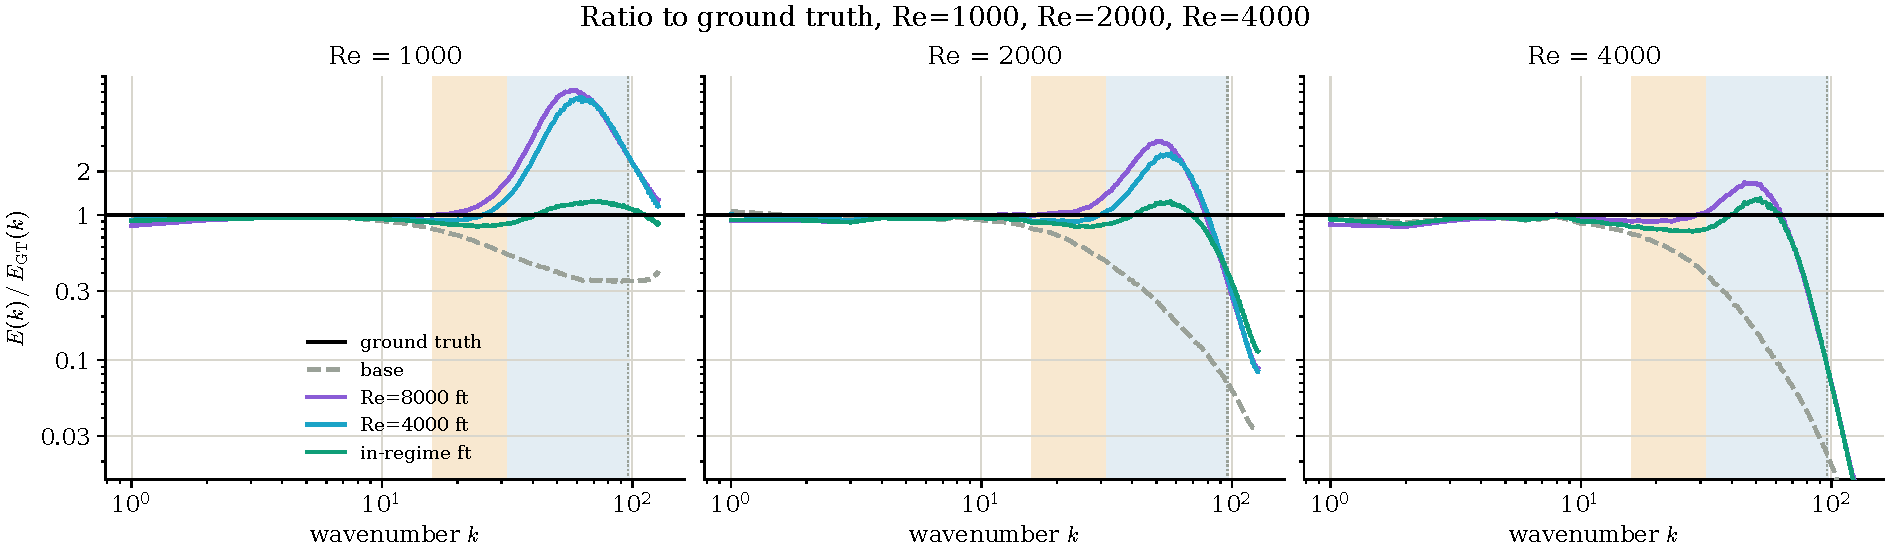
\includegraphics[width=\linewidth]{regime_ratio_dial_lowxfer_low3.pdf}
  \caption{Energy spectrum ratios to ground truth at $Re=1000$, $2000$ and
  $4000$ for the model trained at each regime and the two high regime
  specialists carried in, all under the identical K3 chain. The in regime
  model stays within a small ripple of the truth while the transfers over
  energise the fine scales, by up to seven times at the largest regime gap.}
  \label{fig:lowxfer}
\end{figure}

\begin{table}[t]
  \centering
  \caption{Every specialist at every regime under three mechanisms, as retention over $[32,96)$ with the share of triplets within $\pm20\%$ of their own truth in parentheses. The dial is the tapered guidance at $\lambda=3$; the gate steers each sample toward its own predicted level. For the $Re{=}8000$ model carried below its regime, the chain-shortened sampler replaces guidance: a single $[100]$ chain at $Re{=}1000$ reaches $1.04$ ($70\%$) unguided on the test pool.}
  \label{tab:specialist-transfer-full}
  \begin{tabular}{lrrrrrrr}
    \toprule
    $\mathrm{Re}$ & finetune & ung. & in-b. & $+$dial & in-b. & $+$gate & in-b. \\
    \midrule
    \multirow{4}{*}{1000} & $Re{=}1000$ & 1.00 & 72\% & 1.05 & 44\% & 1.07 & 83\% \\
     & $Re{=}2000$ & 1.58 & 4\% & 1.18 & 39\% & 1.12 & 72\% \\
     & $Re{=}4000$ & 2.83 & 0\% & 1.61 & 10\% & 1.23 & 37\% \\
     & $Re{=}8000$ & 3.71 & 0\% & 2.07 & 1\% & 1.38 & 19\% \\
    \midrule
    \multirow{4}{*}{1500} & $Re{=}1000$ & 0.76 & 40\% & 1.02 & 54\% & 1.08 & 81\% \\
     & $Re{=}2000$ & 1.20 & 49\% & 1.17 & 42\% & 1.16 & 68\% \\
     & $Re{=}4000$ & 2.09 & 1\% & 1.56 & 9\% & 1.28 & 29\% \\
     & $Re{=}8000$ & 2.78 & 0\% & 1.98 & 1\% & 1.45 & 2\% \\
    \midrule
    \multirow{4}{*}{2000} & $Re{=}1000$ & 0.61 & 2\% & 0.86 & 51\% & 0.92 & 95\% \\
     & $Re{=}2000$ & 0.96 & 94\% & 1.00 & 61\% & 1.01 & 95\% \\
     & $Re{=}4000$ & 1.59 & 1\% & 1.30 & 32\% & 1.12 & 80\% \\
     & $Re{=}8000$ & 2.07 & 0\% & 1.61 & 2\% & 1.28 & 26\% \\
    \midrule
    \multirow{4}{*}{3000} & $Re{=}1000$ & 0.48 & 0\% & 0.80 & 45\% & 0.91 & 94\% \\
     & $Re{=}2000$ & 0.75 & 34\% & 0.93 & 64\% & 0.99 & 96\% \\
     & $Re{=}4000$ & 1.20 & 49\% & 1.14 & 54\% & 1.10 & 82\% \\
     & $Re{=}8000$ & 1.59 & 1\% & 1.41 & 21\% & 1.25 & 31\% \\
    \midrule
    \multirow{4}{*}{4000} & $Re{=}1000$ & 0.41 & 0\% & 0.73 & 32\% & 0.87 & 90\% \\
     & $Re{=}2000$ & 0.64 & 5\% & 0.85 & 56\% & 0.94 & 96\% \\
     & $Re{=}4000$ & 1.00 & 74\% & 1.02 & 65\% & 1.03 & 95\% \\
     & $Re{=}8000$ & 1.31 & 31\% & 1.24 & 40\% & 1.17 & 56\% \\
    \midrule
    \multirow{4}{*}{5000} & $Re{=}1000$ & 0.36 & 0\% & 0.64 & 6\% & 0.78 & 42\% \\
     & $Re{=}2000$ & 0.56 & 0\% & 0.75 & 40\% & 0.83 & 70\% \\
     & $Re{=}4000$ & 0.88 & 82\% & 0.90 & 80\% & 0.92 & 92\% \\
     & $Re{=}8000$ & 1.14 & 49\% & 1.08 & 62\% & 1.03 & 91\% \\
    \midrule
    \multirow{4}{*}{6000} & $Re{=}1000$ & 0.36 & 0\% & 0.64 & 18\% & 0.78 & 44\% \\
     & $Re{=}2000$ & 0.55 & 0\% & 0.75 & 36\% & 0.84 & 75\% \\
     & $Re{=}4000$ & 0.86 & 74\% & 0.89 & 71\% & 0.92 & 98\% \\
     & $Re{=}8000$ & 1.10 & 72\% & 1.07 & 68\% & 1.04 & 94\% \\
    \midrule
    \multirow{4}{*}{7000} & $Re{=}1000$ & 0.33 & 0\% & 0.63 & 21\% & 0.80 & 54\% \\
     & $Re{=}2000$ & 0.50 & 0\% & 0.73 & 34\% & 0.86 & 84\% \\
     & $Re{=}4000$ & 0.78 & 49\% & 0.86 & 59\% & 0.92 & 94\% \\
     & $Re{=}8000$ & 1.01 & 72\% & 1.03 & 61\% & 1.03 & 92\% \\
    \midrule
    \multirow{4}{*}{8000} & $Re{=}1000$ & 0.31 & 0\% & 0.58 & 11\% & 0.74 & 21\% \\
     & $Re{=}2000$ & 0.47 & 0\% & 0.68 & 26\% & 0.79 & 49\% \\
     & $Re{=}4000$ & 0.72 & 28\% & 0.79 & 49\% & 0.85 & 74\% \\
     & $Re{=}8000$ & 0.93 & 74\% & 0.95 & 57\% & 0.95 & 100\% \\
    \bottomrule
  \end{tabular}
  \vspace{2pt}\\ \footnotesize Requires \texttt{multirow}.
\end{table}

\begin{table}[t]
  \centering
  \caption{The $Re{=}4000$ and $Re{=}8000$ fine-tunes on the lower half of the ladder under the standard K3 chain, unguided and with the tapered dial at $\lambda=3$, as retention over $[32,96)$ with the share of triplets within $\pm20\%$ of their own truth. The overshoot grows with the distance below the training regime and the dial reduces it by roughly half without landing it, for both models.}
  \label{tab:downward-4k8k}
  \begin{tabular}{lrrrrrrrr}
    \toprule
    $\mathrm{Re}$ & 4k ung. & in-b. & 4k $+$dial & in-b. & 8k ung. & in-b. & 8k $+$dial & in-b. \\
    \midrule
    1000 & 2.83 & 0\% & 1.61 & 10\% & 3.71 & 0\% & 2.07 & 1\% \\
    1500 & 2.09 & 1\% & 1.56 & 9\% & 2.78 & 0\% & 1.98 & 1\% \\
    2000 & 1.59 & 1\% & 1.30 & 32\% & 2.07 & 0\% & 1.61 & 2\% \\
    3000 & 1.20 & 49\% & 1.14 & 54\% & 1.59 & 1\% & 1.41 & 21\% \\
    4000 & 1.00 & 74\% & 1.02 & 65\% & 1.31 & 31\% & 1.24 & 40\% \\
    \bottomrule
  \end{tabular}
\end{table}

\begin{table}[t]
  \centering
  \caption{Where the downward surplus lives in wavenumber. Low-$k$ is retention over $[1,5)$; onset is the first shell whose energy exceeds the truth and stays above it; the last column is where the ratio returns under $1$. The large scales are preserved within a few percent everywhere while the surplus onset retreats toward higher $k$ as the target approaches the training regime.}
  \label{tab:overshoot-onset}
  \begin{tabular}{lrrrrr}
    \toprule
    $\mathrm{Re}$ & model & low-$k$ & onset $k$ & peak & under $1$ at \\
    \midrule
    1000 & $Re{=}4000$ ft & 0.98 & 26 & 6.5$\times$ at 62 & never \\
     & $Re{=}8000$ ft & 0.96 & 17 & 7.2$\times$ at 57 & never \\
    2000 & $Re{=}4000$ ft & 0.98 & 30 & 2.6$\times$ at 57 & 81 \\
     & $Re{=}8000$ ft & 0.95 & 17 & 3.2$\times$ at 52 & 79 \\
    4000 & $Re{=}4000$ ft & 0.98 & 40 & 1.3$\times$ at 52 & 61 \\
     & $Re{=}8000$ ft & 0.95 & 29 & 1.7$\times$ at 45 & 63 \\
    \bottomrule
  \end{tabular}
\end{table}


\begin{figure}[t]
  \centering
  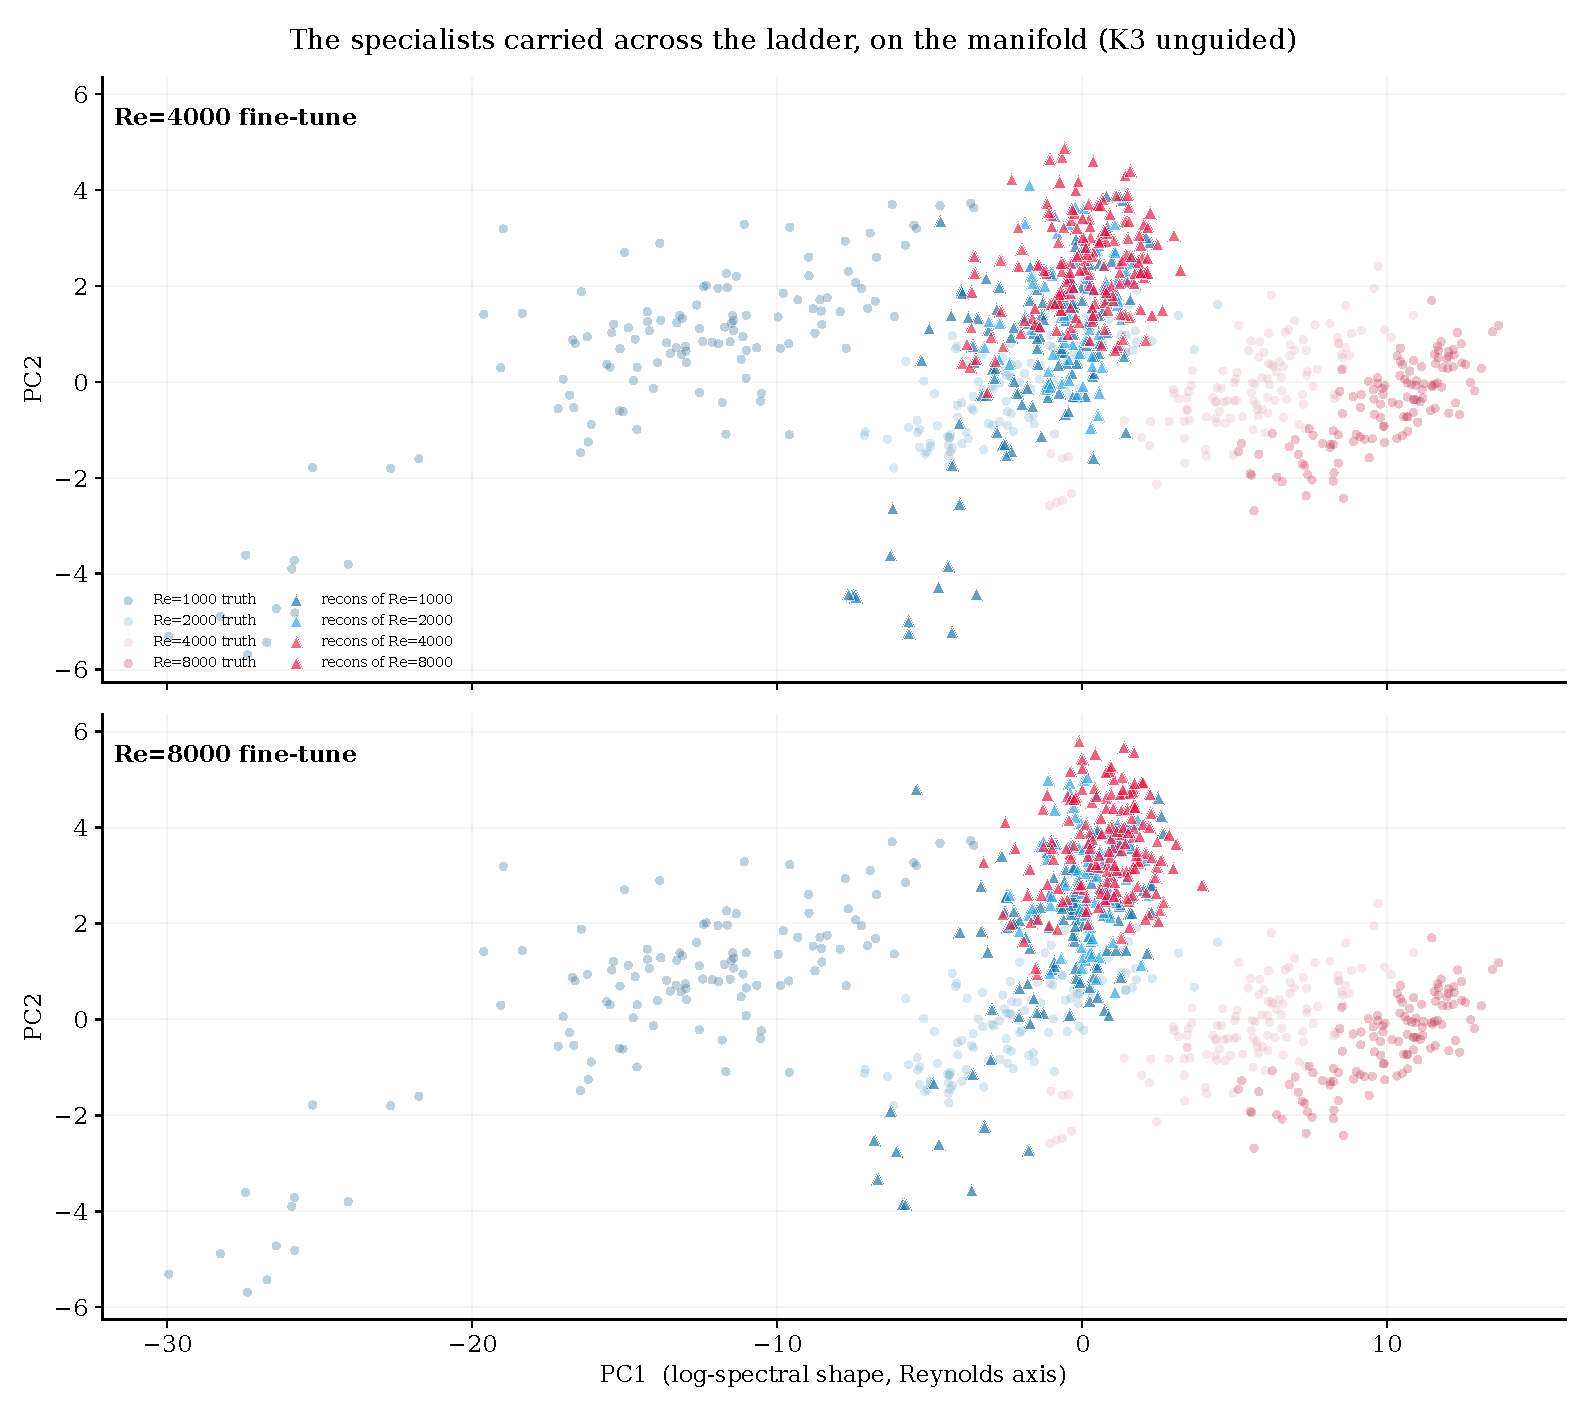
\includegraphics[width=\linewidth]{manifold_transfer_clouds.pdf}
  \caption{The two high regime specialists carried across the ladder, on the
  spectral manifold. Triangles are reconstruction clouds coloured by their
  target regime and are read against the truth cloud of the same colour. Under
  fixed inference each model drags every input to essentially one destination,
  so the transfer error at a rung is the distance from that destination to the
  rung's truth.}
  \label{fig:transfer-clouds}
\end{figure}

% ----------------------------------------------------------------------------
\subsection{What the specialists share}
\label{sec:transfer-shared}

The sampler interacts with the learned weights through a single quantity, the
noise prediction $\epsilon_\theta$. Whatever fine tuning changed is therefore
fully contained in the difference between a specialist's prediction and the
base model's prediction on identical inputs, and this difference can be
measured directly. Probing it on matched noised samples separates what the
specialists learned from how the sampler happens to use it, and the answer
turns out to be simple.

The corrections of the specialists occupy the same locations and point in the
same direction. Their spatial supports overlap by roughly one half, the cosine
similarity between the corrections of different specialists on the same input
lies between $0.55$ and $0.64$, and close to half of the strongest correction
is explained by the linear span of the two weaker ones
(Figure~\ref{fig:eps-maps}, Table~\ref{tab:eps-stats}). Seen as maps, the
corrections sharpen the same filaments and deepen the same vortex cores, and a
reader shown the three maps without labels would order them by intensity rather
than sort them by content.

What distinguishes the specialists is magnitude and spectral reach. The
correction norms are ordered as $1$ to $1.38$ to $2.29$ across the training
regimes, and the fraction of correction power carried above $k=32$ grows from
$0.58$ to $0.70$ in the same order. A higher regime specialist is to first
order a stronger and slightly finer grained version of a lower regime one, and
the part of its correction that the weaker models do not share lives almost
entirely in the fine scales.

Fine tuning has therefore re weighted a shared correction rather than learned
regime specific physics. The models appear to exploit the common large scale
structure of Kolmogorov flows, which changes little across the ladder, and
differ in how strongly they energise its fine scales. This is the observation
that makes an inference time remedy plausible. A difference of kind would
demand different weights for every regime, but a difference of degree can be
dosed.

\begin{figure}[t]
  \centering
  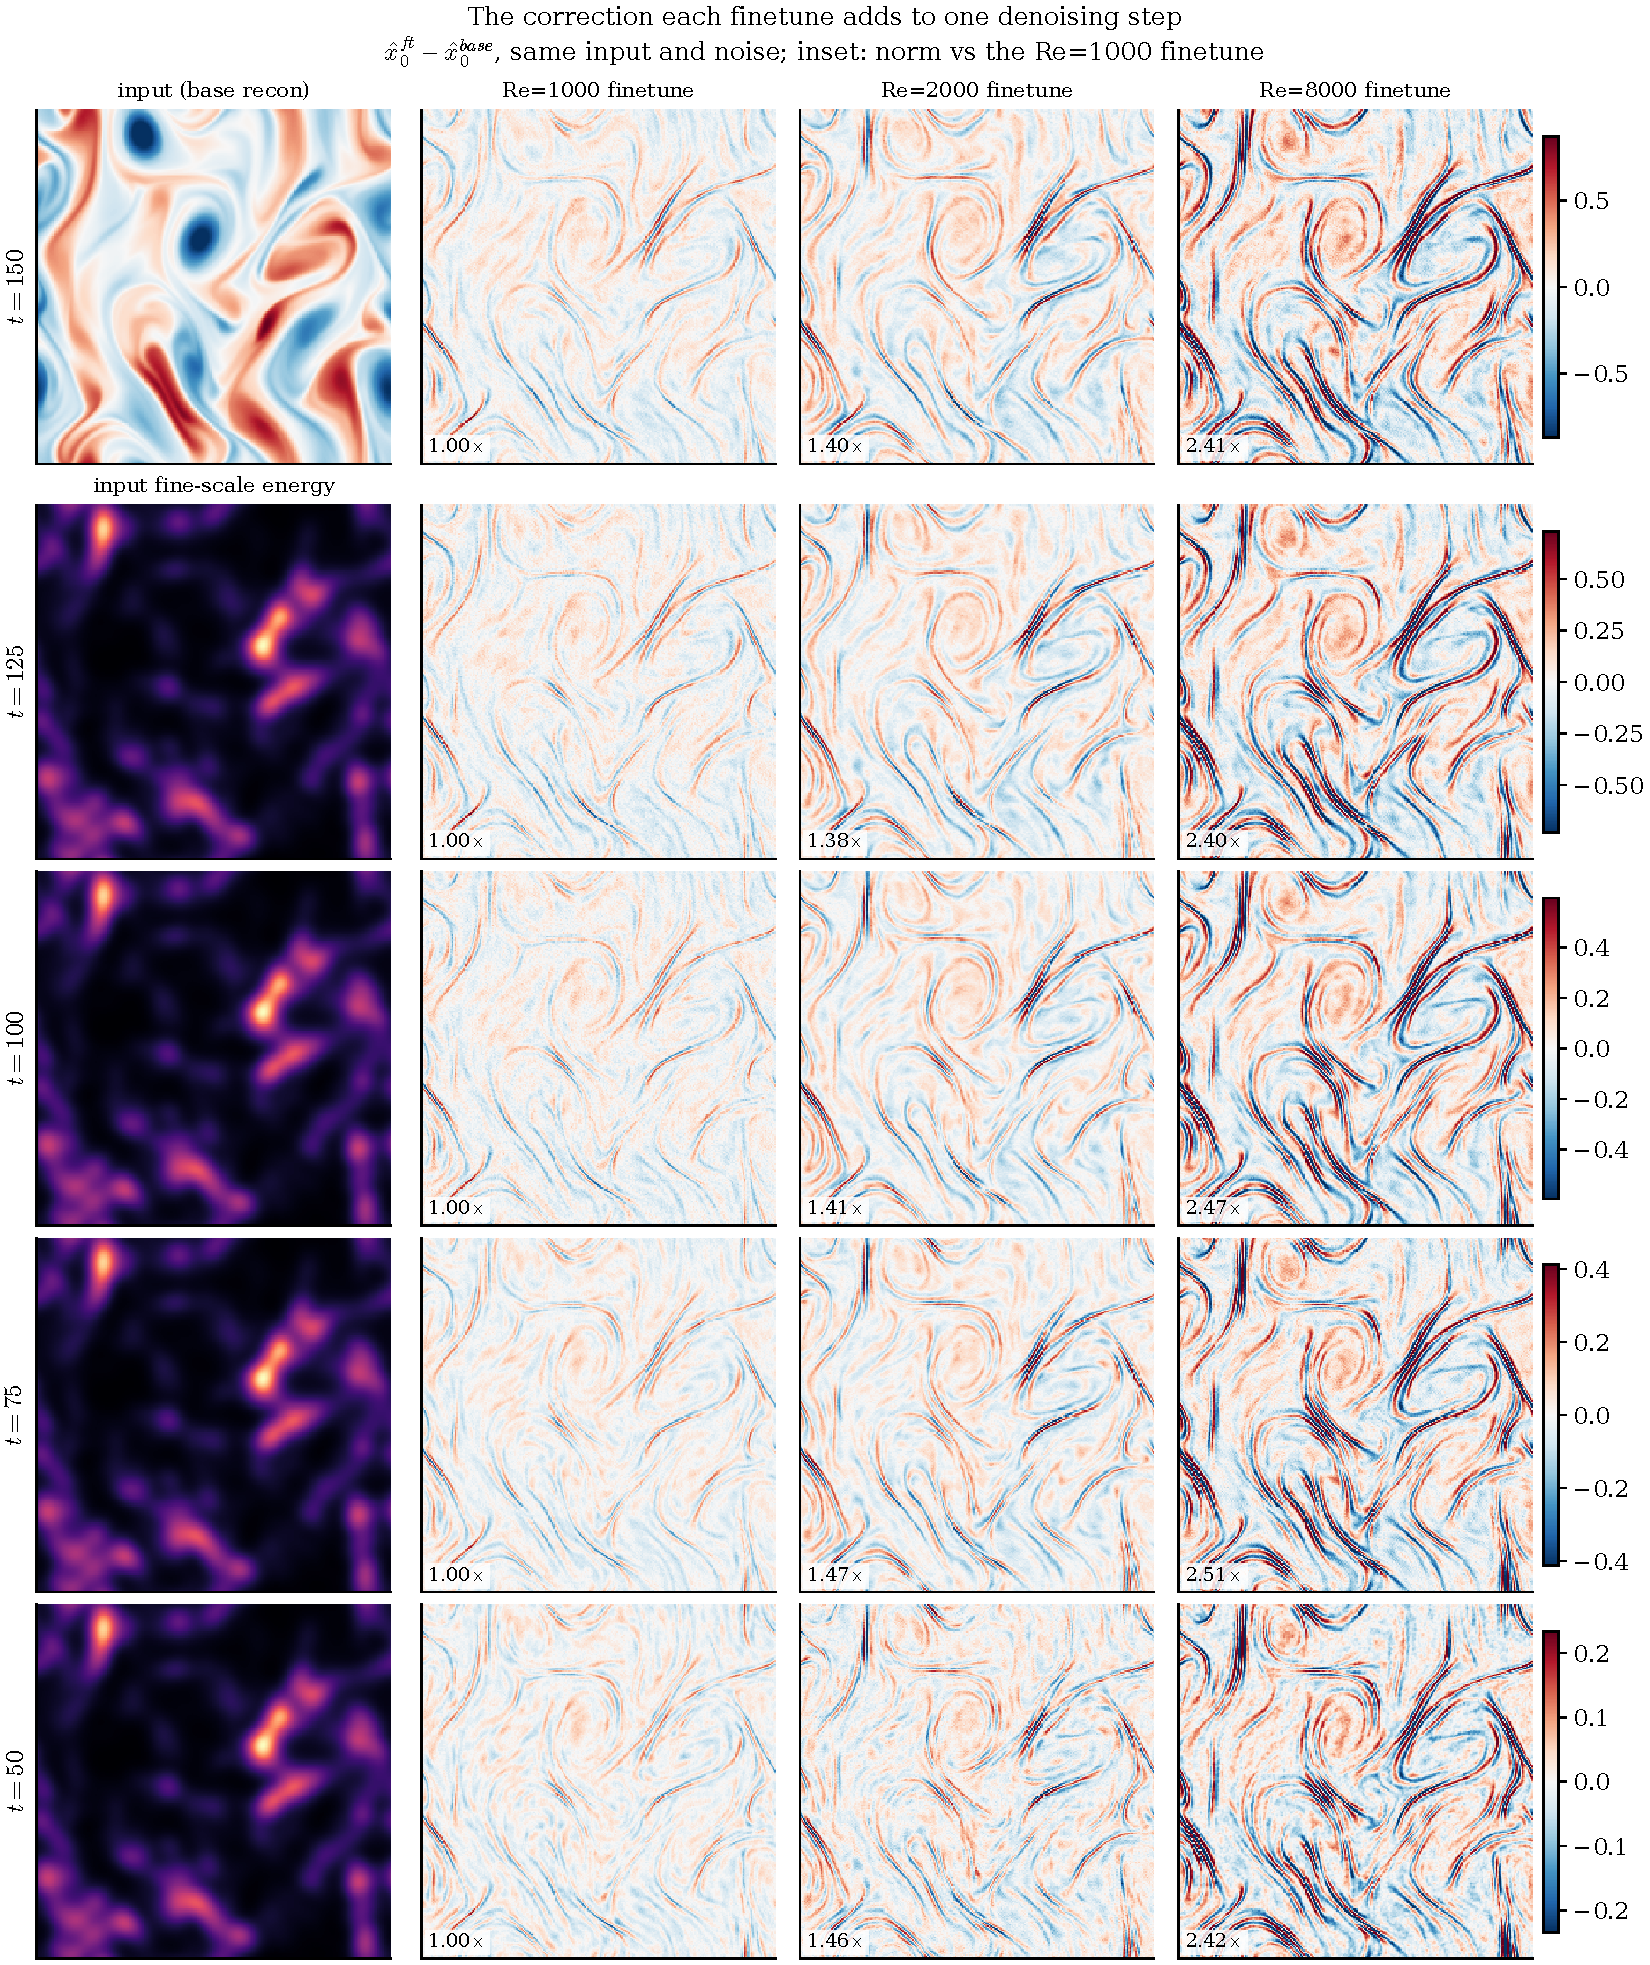
\includegraphics[width=\linewidth]{eps_correction_maps.pdf}
  \caption{Single step corrections $d\hat{x}_0$ of the fine tuned models on
  identical noised inputs, at five noise levels. The corrections act in the
  same places and differ chiefly in amplitude, with the higher regime models
  reaching further into the fine scales.}
  \label{fig:eps-maps}
\end{figure}

\begin{table}[t]
  \centering
  \caption{Statistics of the single-step correction $\Delta\epsilon=\epsilon_{ft}-\epsilon_{base}$ on identical noised inputs from the $Re{=}1000$ test pool, per sample, over $t\in\{150,100,50\}$ and two noise draws ($36$ cells). The $Re{=}1000$ finetune's correction carries a $k\geq32$ power fraction of 0.58 $\pm$ 0.05.}
  \label{tab:eps-correction-stats}
  \begin{tabular}{lrr}
    \toprule
    & $Re{=}2000$ ft & $Re{=}8000$ ft \\
    \midrule
    $\|\Delta\epsilon\|$ vs $Re{=}1000$ ft & 1.38 $\pm$ 0.10 & 2.29 $\pm$ 0.19 \\
    cosine with $Re{=}1000$ ft & 0.53 $\pm$ 0.09 & 0.55 $\pm$ 0.07 \\
    cosine $Re{=}8000$ vs $Re{=}2000$ &  & 0.64 $\pm$ 0.09 \\
    variance explained by span of the other two &  & 0.47 $\pm$ 0.10 \\
    support overlap of $|\Delta\epsilon|$ with $Re{=}1000$ ft & 0.48 $\pm$ 0.09 & 0.51 $\pm$ 0.07 \\
    fraction of correction power at $k\geq32$ & 0.64 $\pm$ 0.07 & 0.70 $\pm$ 0.06 \\
    \bottomrule
  \end{tabular}
\end{table}


% ----------------------------------------------------------------------------
\subsection{The mechanism of dose delivery}
\label{sec:transfer-mechanism}

Two complementary instruments are used in this part. The first records the
fine band energy of the running clean estimate at every step of the sampling
chain, and answers when the dose is delivered. The second embeds
reconstructions in a low dimensional spectral manifold, built from a principal
component analysis of per sample log spectra over the pooled ground truths of
four regimes, and answers where the sample travels. The leading component of
this embedding orders the regimes and carries 96 percent of the variance, so
trajectories through the space can be read as movement along a Reynolds axis.
The projection collapses spectral shape to a coordinate, so proximity in the
embedding is a necessary rather than a sufficient condition for spectral
agreement, and every claim made on the manifold in this section is paired with
a claim made on the spectra themselves.

The dose is set at the first clean estimate of each pass. Relative to the
reconstruction the chain starts from, the first estimate of the first pass
multiplies the fine band energy by $1.64$ for the $Re=1000$ fine tune, $2.05$
for $Re=2000$, $3.01$ for $Re=4000$ and $3.63$ for $Re=8000$, while the base
model multiplies it by $1.03$ (Figure~\ref{fig:energy-trace},
Table~\ref{tab:chain-injection}). The remaining nineteen steps of the pass
change the level by between eight and twenty five percent, and they do so
almost identically for every model. The refinement phase carries essentially
no model identity. Each renoising then repeats the injection at a smaller
scale, with the $Re=8000$ multipliers falling from $3.63$ at depth $150$ to
$2.04$ at depth $100$ and $1.33$ at depth $50$, so the total dose is a
function of the model and of the renoising schedule and of nothing else.

A deterministic and a stochastic rendering of the same chain separate the
model's injection from the sampler's. Under deterministic steps the picture
above is exact and every curve lands low, while under the production sampler
the same seeds and sample carry each model to the level its aggregate test
statistics predict, with the $Re=1000$ fine tune finishing on its truth line.
The gap between the two renderings is the energy contributed by the sampling
noise itself, and it accounts for roughly a third of the delivered dose at
$Re=1000$. The deterministic trace is the dissection and the stochastic trace
is the deployment, and the pair is shown together because the difference
between them is itself a finding.

The magnitude of the learned correction is nearly constant through the chain.
Measured on each model's own states against the base prediction on the same
input, the per pass mean of the correction norm changes by less than fifteen
percent between the three passes, while relative to the base score the
correction grows from about ten percent early in a pass to between thirty and
fifty percent at its end (Figure~\ref{fig:eps-norms}). The model is not
predicting less as the chain descends. The shrinking dose of later passes is a
property of the sampler geometry, which scales how a fixed size correction
reaches the clean estimate.

The manifold shows what this machinery does to the actual sample. Renoising to
depth $150$ moves the state to a single point far off the manifold, identical
for every model because the noise is shared, and further along the Reynolds
axis than any true regime because white noise carries a flat spectrum that
impersonates fine scale turbulence (Figure~\ref{fig:pass1}). From that shared
launch the five models walk back along five different arcs. The base model
identifies the added energy as noise and removes it, returning almost exactly
to the reconstruction it started from, which is precisely why it cannot
transfer. Each specialist instead retains a trained fraction of the injected
energy as coherent structure, and the retained fraction, ordered by training
regime, is the dose.

The moves of successive passes shrink in a fixed proportion. Along the
Reynolds axis the $Re=8000$ model advances fourteen units in the first pass,
three and a half in the second and essentially nothing in the third, and every
other fine tune shows the same collapse at its own scale
(Table~\ref{tab:manifold-pass-distances}). Within a pass the number of
denoising steps changes the endpoint by almost nothing. The leverage over the
dose therefore lies in the renoise depth and the number of passes, which is
the operational content of the claim that the chain is the dose.

Finally, the starting point of the journey barely depends on the regime of the
input. The base reconstructions of all four regimes crowd into one
neighbourhood of the manifold, with median first coordinates between $-19.8$
and $-12.5$, a span of seven units against the twenty three spanned by the
truths (Figure~\ref{fig:recon-starts}). The standard reconstruction is a great
equaliser, rendering roughly base level fine scale content whatever it is
given, so the travel required of the chain is set almost entirely by where the
target truth lives. The required journey grows from seven units at $Re=1000$
to twenty three at $Re=8000$, while the vehicle and its starting point stay
the same.

\begin{figure}[t]
  \centering
  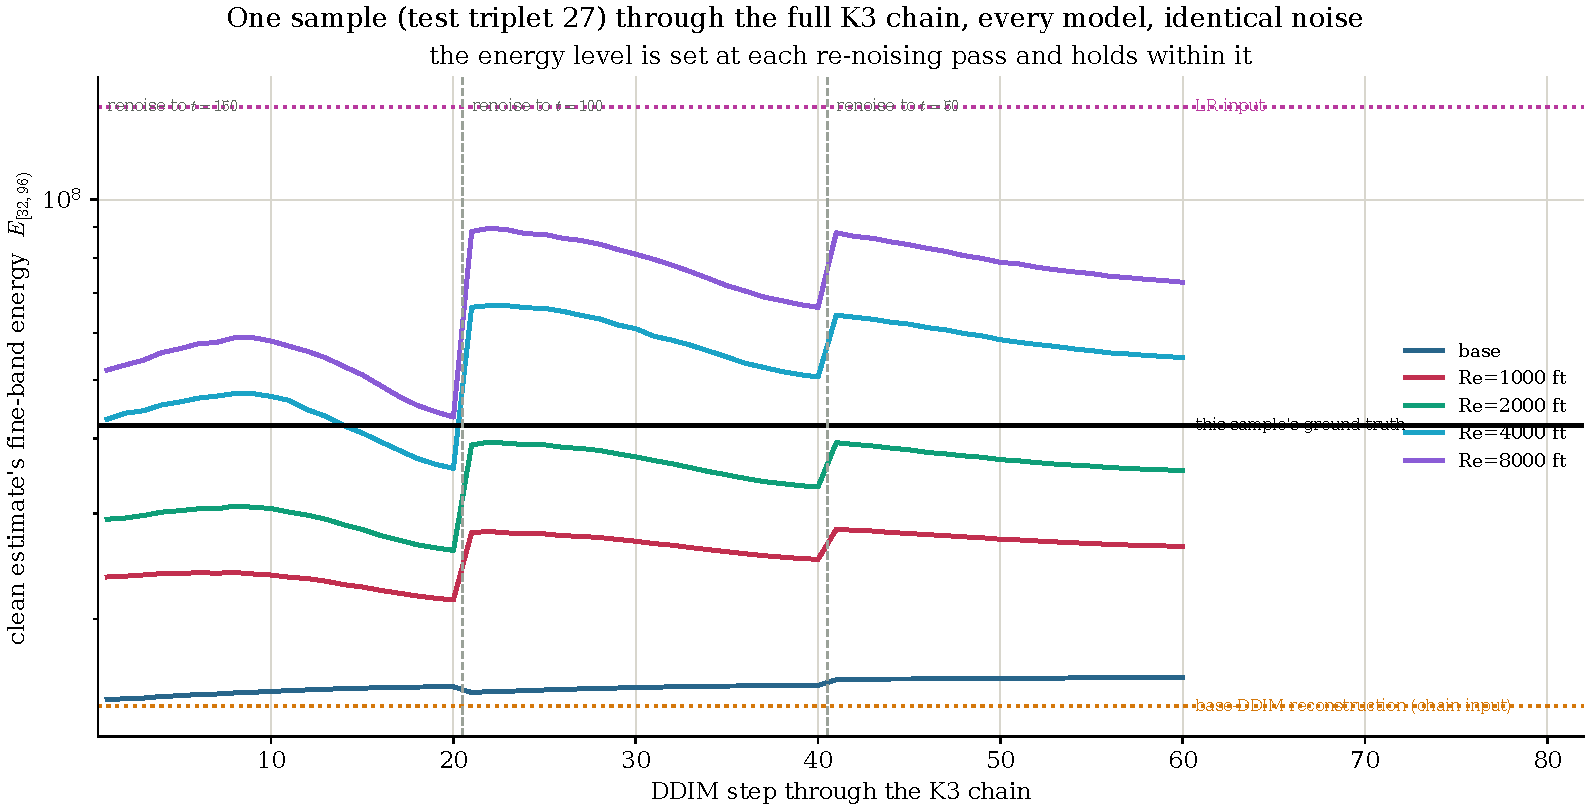
\includegraphics[width=\linewidth]{chain_energy_trace.pdf}\\
  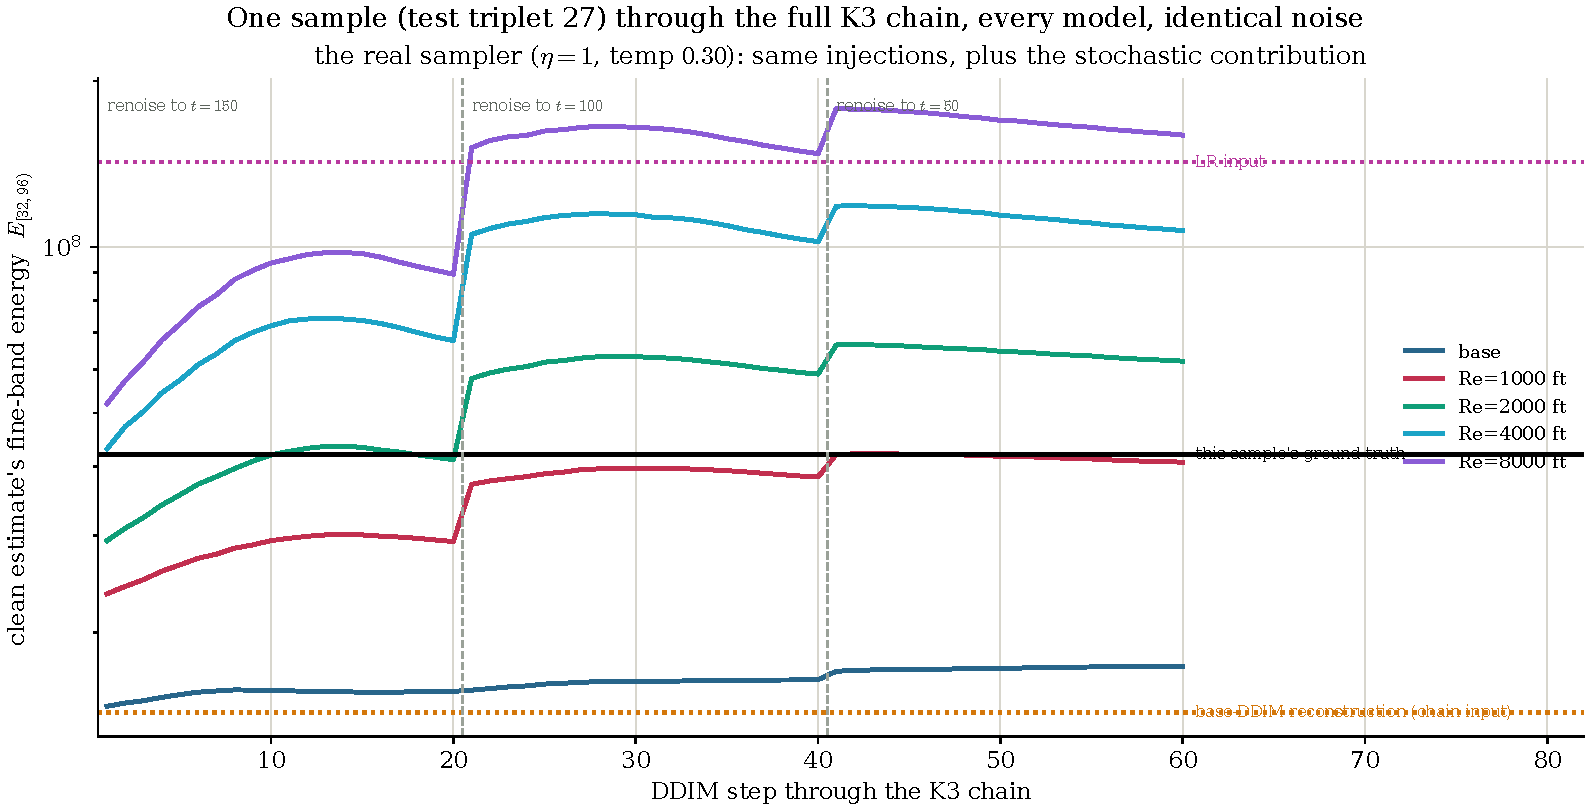
\includegraphics[width=\linewidth]{chain_energy_trace_eta1.pdf}
  \caption{One test sample through the full K3 chain, every model, identical
  noise. Top, deterministic steps isolate the model's injection, which
  arrives at the first clean estimate of each pass and is ordered by training
  regime. Bottom, the real stochastic sampler on the same sample and seeds.
  The gap between the panels is the energy contributed by the sampling noise,
  and under the real sampler the $Re=1000$ fine tune finishes on its truth
  line while the others land in the order of their training regimes.}
  \label{fig:energy-trace}
\end{figure}

\begin{table}[t]
  \centering
  \caption{Fine-band energy $E_{[32,96)}$ multipliers through the K3 chain at $Re{=}1000$, one sample, identical noise across models. Step 1 is the first clean estimate relative to the reconstruction the chain starts from; each drift column is the change over the remaining steps of that pass; each jump is the change across a renoising. The dose is set at the first estimate of each pass and the refinement phase is nearly flat, so total dose is a function of the model and the renoising schedule, not of the step count.}
  \label{tab:chain-injection}
  \begin{tabular}{lrrrrrr}
    \toprule
    model & step 1 / input & rest of pass 1 & jump 2 & drift 2 & jump 3 & drift 3 \\
    \midrule
    base & 1.03 & 1.05 & 0.98 & 1.03 & 1.02 & 1.01 \\
    $Re{=}1000$ ft & 1.64 & 0.92 & 1.30 & 0.90 & 1.12 & 0.94 \\
    $Re{=}2000$ ft & 2.05 & 0.89 & 1.50 & 0.85 & 1.19 & 0.90 \\
    $Re{=}4000$ ft & 3.01 & 0.83 & 1.86 & 0.77 & 1.27 & 0.85 \\
    $Re{=}8000$ ft & 3.63 & 0.84 & 2.04 & 0.75 & 1.33 & 0.83 \\
    \bottomrule
  \end{tabular}
\end{table}


\begin{figure}[t]
  \centering
  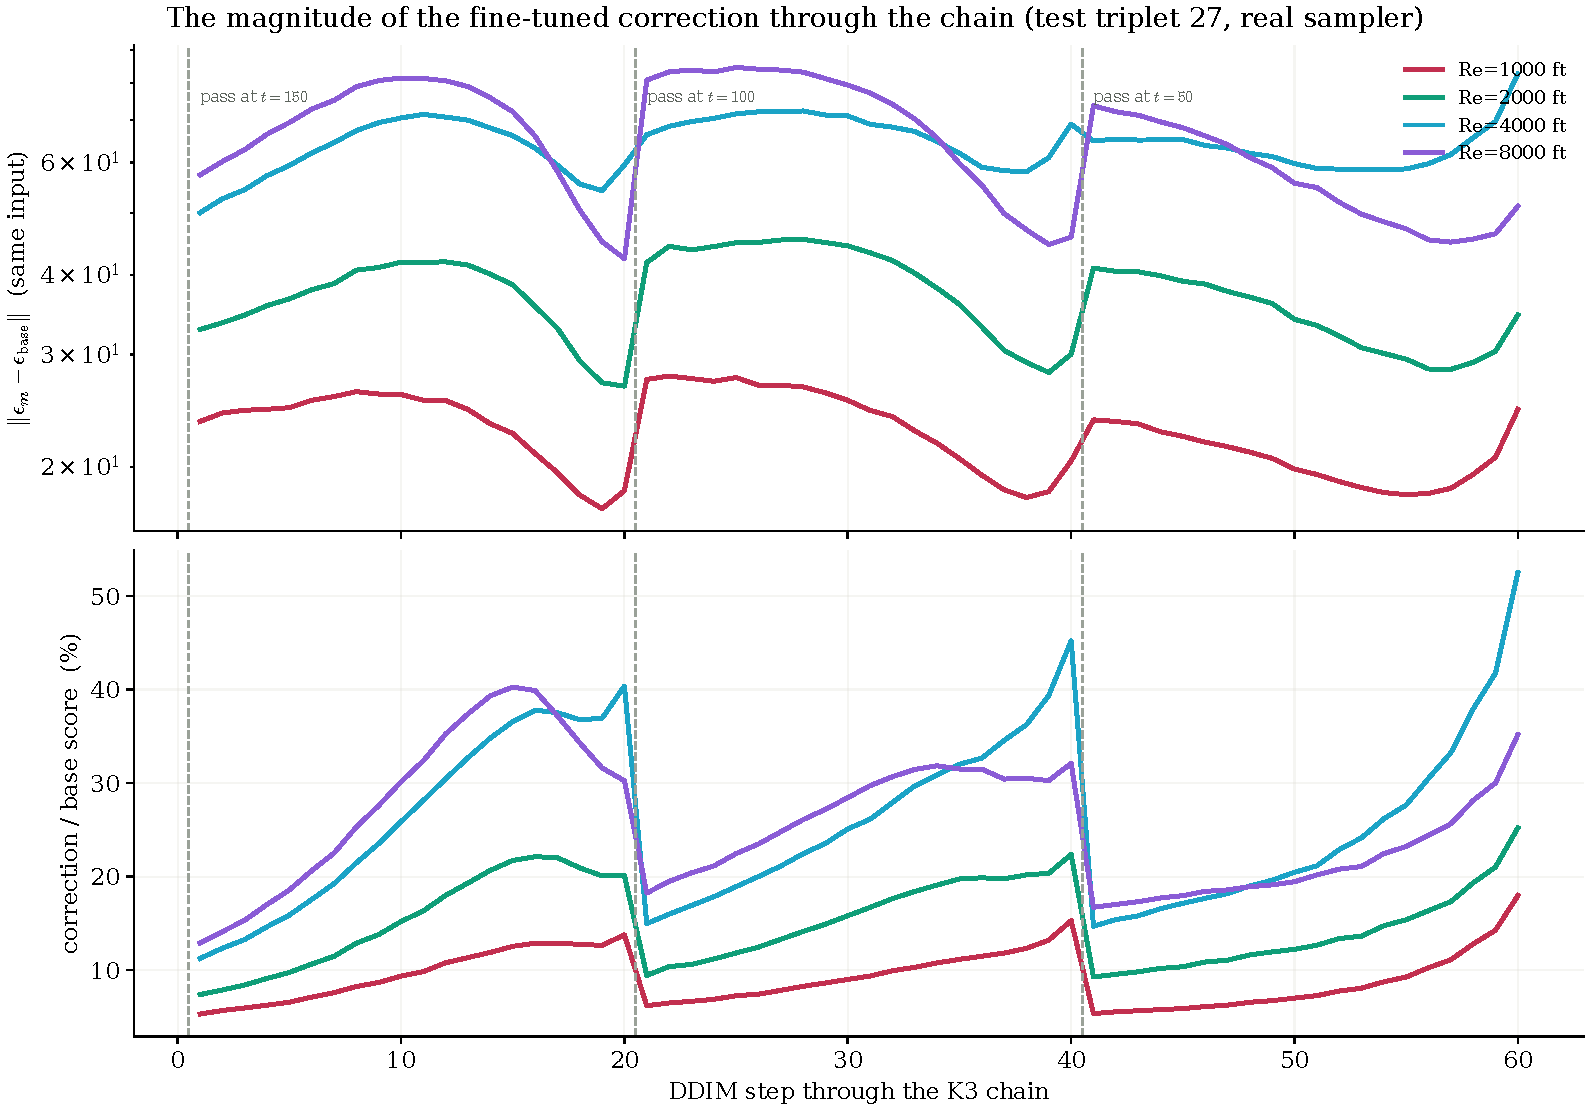
\includegraphics[width=\linewidth]{eps_chain_norms.pdf}
  \caption{Norm of the fine tuned correction along each model's own chain,
  measured against the base prediction on the same input, absolute and
  relative to the base score. The correction breathes within a pass but its
  pass means barely move, and relative to the base score it grows toward the
  end of each pass.}
  \label{fig:eps-norms}
\end{figure}

\begin{figure}[t]
  \centering
  
\includegraphics[width=\linewidth]{offmanifold_pass1.pdf}
  \caption{The actual state $x_t$ through the first pass at the $Re=1000$
  target. Renoising teleports the sample to a single shared point far off the
  manifold, and each model walks it back along its own arc. The base returns
  almost exactly to the reconstruction it started from, while the specialists
  retain a trained fraction of the injected energy.}
  \label{fig:pass1}
\end{figure}

\begin{table}[t]
  \centering
  \caption{Net displacement along the Reynolds axis (PC1 of the log-spectral basis) produced by each pass of the K3 chain, from the state entering the pass to its final clean estimate, mean $\pm$ sd over one median sample at each of the four embedded regimes, identical noise across models. The move shrinks with the renoise depth $t$ for every model, and at fixed $t$ grows with the training regime.}
  \label{tab:manifold-pass-distances}
  \begin{tabular}{lrrr}
    \toprule
    model & pass 1 ($t{=}150$) & pass 2 ($t{=}100$) & pass 3 ($t{=}50$) \\
    \midrule
    base & $-2.1 \pm 1.7$ & $+1.6 \pm 0.2$ & $+0.8 \pm 0.0$ \\
    $Re{=}1000$ ft & $+4.3 \pm 2.5$ & $+2.9 \pm 0.4$ & $+0.5 \pm 0.1$ \\
    $Re{=}2000$ ft & $+9.5 \pm 2.6$ & $+3.5 \pm 0.6$ & $+0.4 \pm 0.0$ \\
    $Re{=}4000$ ft & $+13.4 \pm 3.3$ & $+3.5 \pm 0.5$ & $+0.1 \pm 0.1$ \\
    $Re{=}8000$ ft & $+14.0 \pm 3.5$ & $+3.4 \pm 0.5$ & $+0.2 \pm 0.0$ \\
    \bottomrule
  \end{tabular}
\end{table}


\begin{figure}[t]
  \centering
  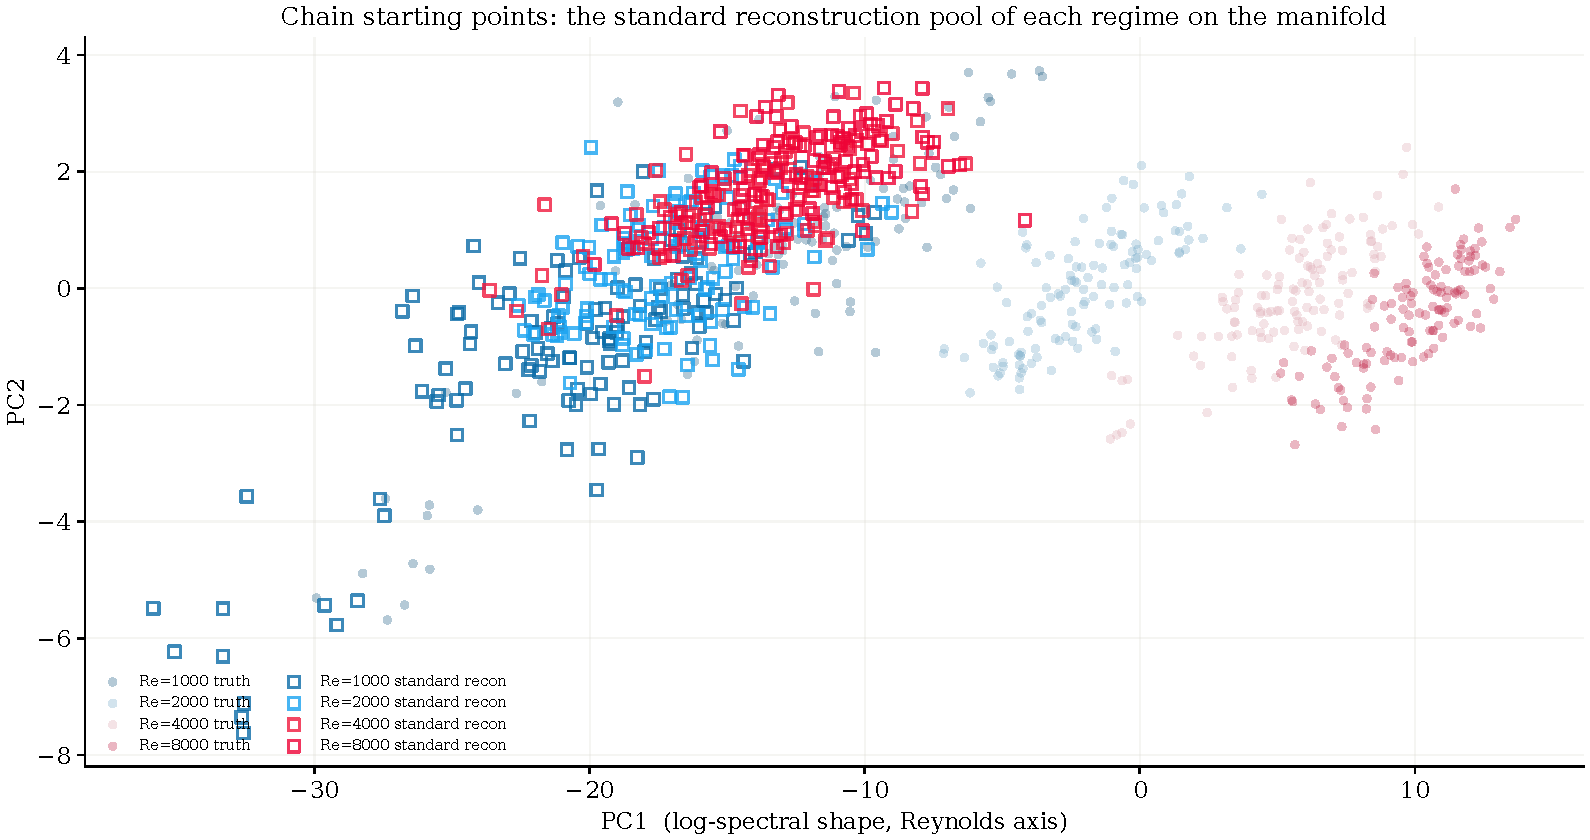
\includegraphics[width=\linewidth]{manifold_recon_starts.pdf}
  \caption{The standard reconstruction pool of each regime on the manifold.
  The truths span twenty three units along the Reynolds axis while their
  reconstructions span seven, so the chain starts from nearly the same place
  whatever the regime of the input, and the required travel is set by the
  target.}
  \label{fig:recon-starts}
\end{figure}

% ----------------------------------------------------------------------------
\subsection{Adaptive inference with fixed weights}
\label{sec:transfer-adaptive}

The mechanism licenses a fix. If the dose is a monotone function of the
renoise depth and the pass count, and the transfer error is a monotone
function of the distance below the training regime, then a per regime schedule
of the chain should land every rung without touching the weights. Selecting a
chain requires no paired ground truth samples. The retention it optimises
compares the ensemble band energy of the candidate reconstructions with the
ensemble spectral statistics of the target flow, the same quantity the reward
is anchored to, and a practitioner could obtain it from a short reference
simulation of the regime. We measure these statistics on the held out
validation split, evaluate every candidate chain there, and spend the test
pool exactly once on the selected configuration. The provenance of the
reference statistics does matter. A variant of the rule anchored to the
training split was also evaluated, and its proxies inherit offsets of up to
twelve percent from split to split scatter in the large scales, enough to
reject working chains at the intermediate regimes. The reference must
therefore be measured on a pool representative of the flows being
reconstructed, and this requirement is the practical boundary of the method
rather than a need for ground truth pairs.

Removing passes and then reducing the renoise depth walks the same sample back
across the manifold in controlled steps
(Figure~\ref{fig:dechain}). Because the shortened chains share the noise
sequence of the full one, dropping a pass is literally stopping the same
trajectory at an earlier renoising, and the reader can verify on the figure
that the second and third passes are where the transfer surplus comes from.
Reducing the depth of the single remaining pass then walks the endpoint the
rest of the way in small steps.

The selected rungs form an almost regular ladder. A single pass at depth
$100$ lands $Re=1000$ with retention $1.04$ and seventy percent of samples in
band, depth $120$ lands $Re=1500$ at $1.10$, depth $125$ lands $Re=2000$ at
$0.93$ with ninety four percent in band, depth $150$ lands $Re=3000$ at
$0.97$, and depth $160$ lands $Re=4000$ at $0.90$
(Table~\ref{tab:re8k-downward}). Each rung was selected on validation and
confirmed once on test. The regularity of the ladder is itself evidence for
the dose law of the previous part, since a smooth monotone map from renoise
depth to delivered energy is exactly what that law predicts.

The two halves of the ladder call for different tools. Below the training
regime the chain is the mechanism, because guidance cannot suppress an
overdose approaching four times the truth, and the best guided full chain
still retains $1.38$ at $Re=1000$ where the plain shortened chain reaches
$1.04$. At and above the training regime there is no deeper chain to reach
for, the full chain is the correct depth, and guidance provides the remaining
lift (Figure~\ref{fig:bestconfig}). The tapered dial composes with a tuned
chain as a signed per sample corrector. It pulls a small surplus down, from
$1.04$ to $0.96$ at $Re=1000$, and pushes a small deficit up, from $0.90$ to
$0.95$ at $Re=4000$, the direction flipping automatically because the dial
steers toward a target level rather than injecting blindly. The correction
costs some per sample placement below the training regime, so the bare chain
remains preferable where its dose is already right.

One model therefore reaches every rung of the ladder to within seven percent
of the true band energy, with the chain carrying the lower half and the gate
of the next part carrying the upper half
(Figure~\ref{fig:bestconfig-spectra}). What no configuration changes is the
highest octave. In every setting the reconstruction leaves the truth line for
good between $k$ of roughly $55$ and $75$ and collapses by $k$ near $100$, at
its home regime as much as in transfer. Inference adaptation solves the dose,
and the last octave remains a property of the model that no schedule or
guidance strength recovers. It marks the boundary between what this section
can fix and what must be fixed in the weights.

\begin{figure}[t]
  \centering
  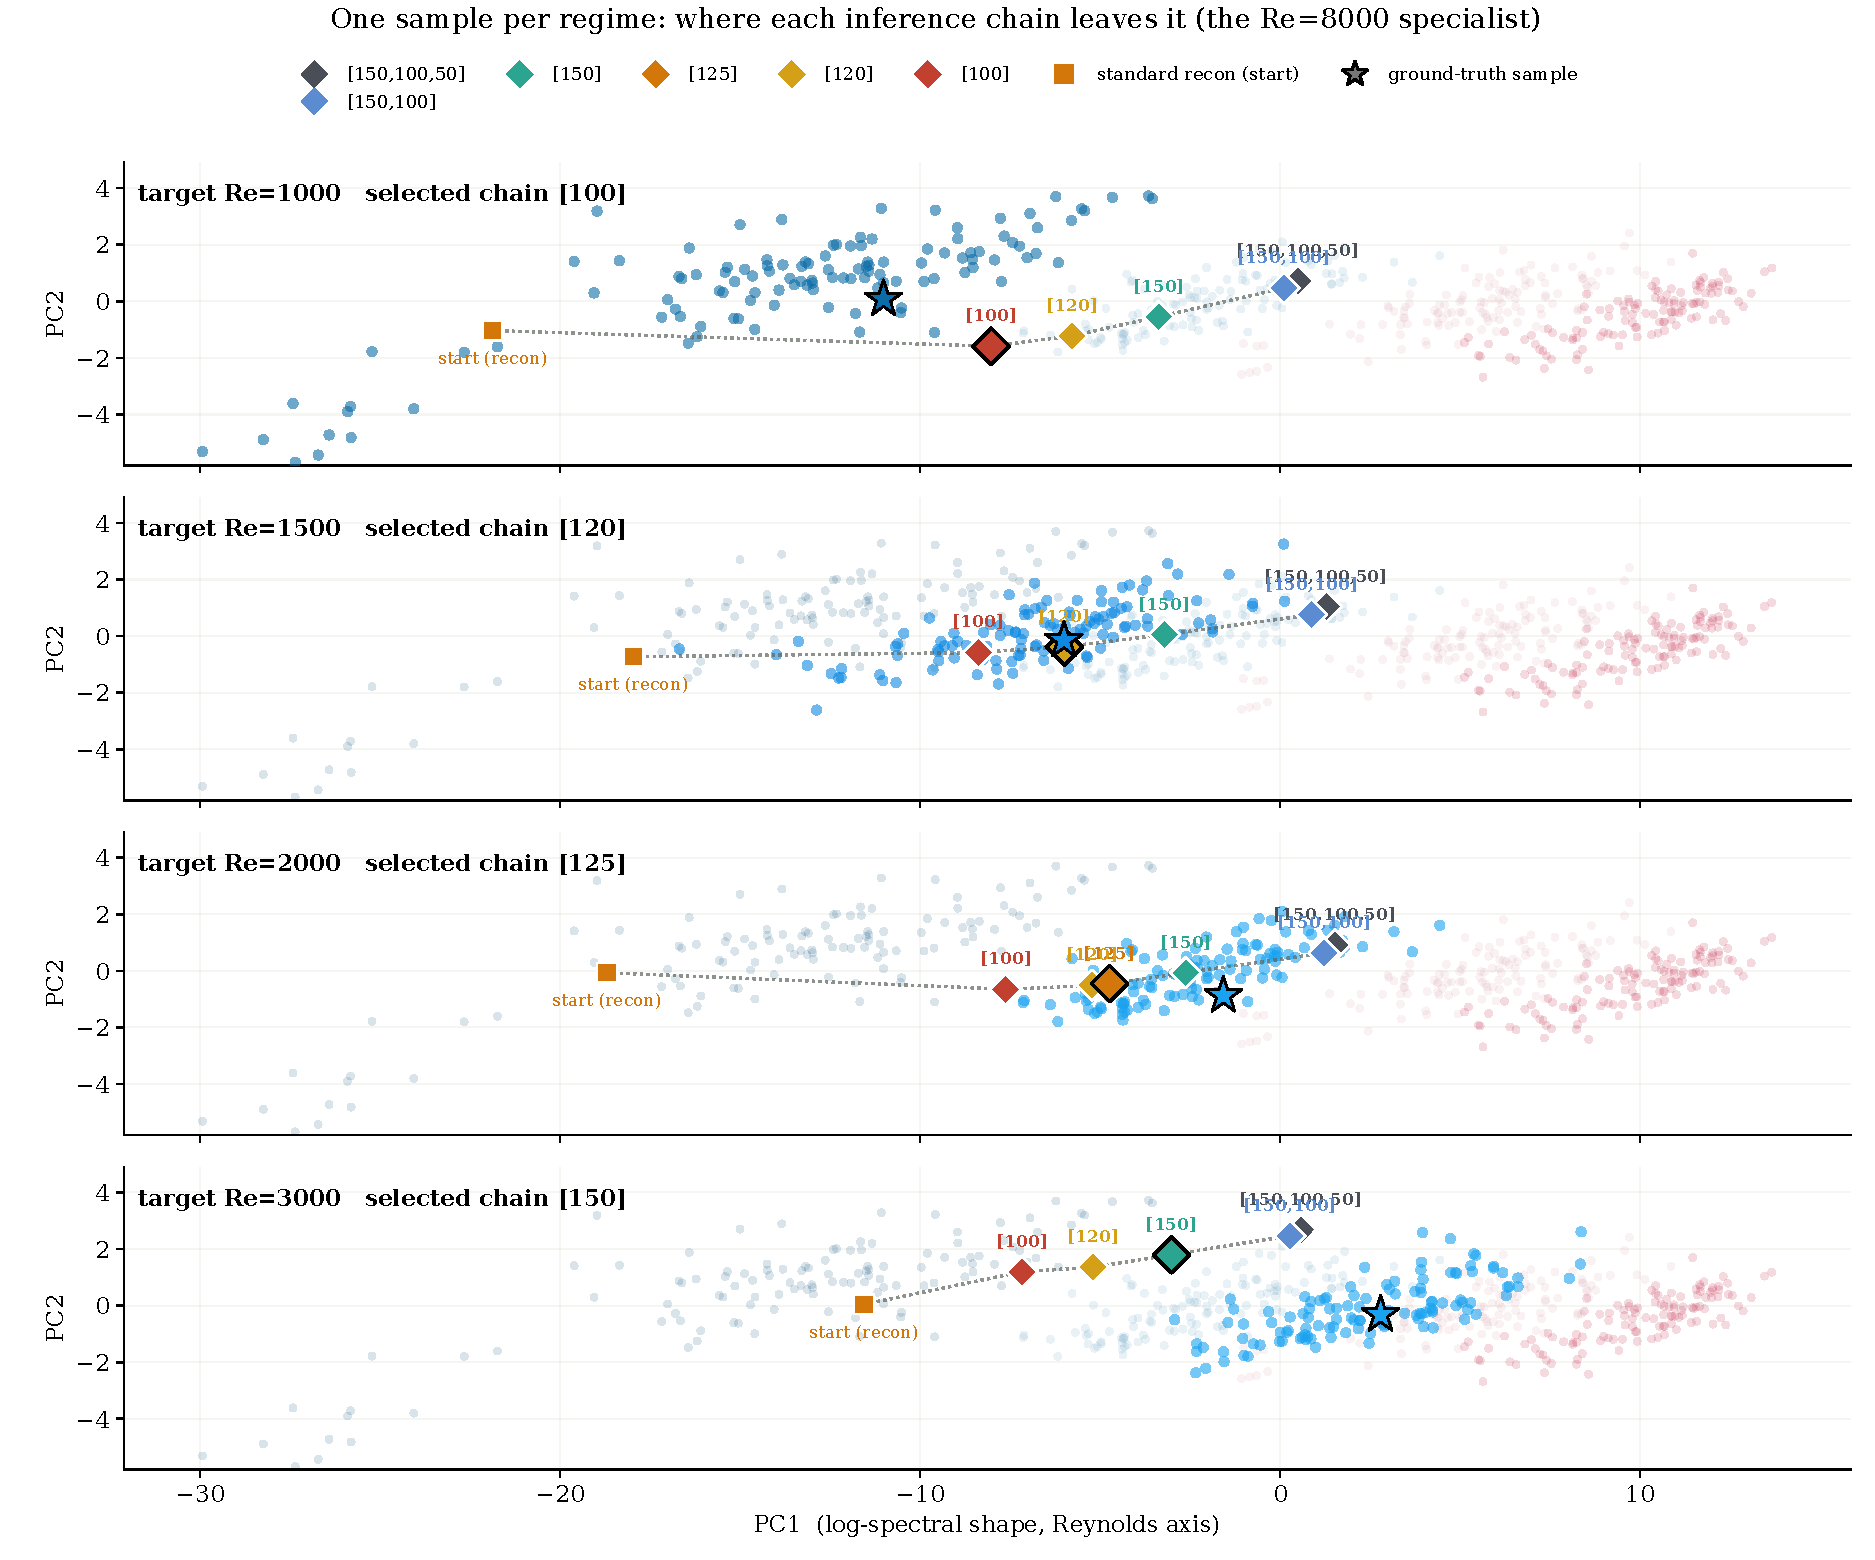
\includegraphics[width=\linewidth]{offmanifold_dechain_endpoints.pdf}
  \caption{One sample per downward regime, where each inference chain leaves
  it. Dropping passes and then reducing the renoise depth marches the
  endpoint back from the model's fixed destination onto the target cloud, and
  the selected chain lands on or beside the sample's own truth in every
  panel.}
  \label{fig:dechain}
\end{figure}

\begin{table}[t]
  \centering
  \caption{The $Re{=}8000$ finetune carried down the regime ladder: retention over $[32,96)$ and the share of triplets within $\pm20\%$ of their own truth, under the standard K3 chain (unguided, tapered dial at $\lambda=3$, and the target-gated dial), and with the chain-shortened sampler, unguided, where a rung has been evaluated on the test pool. Each chain is selected per regime on the validation pool before the single test evaluation. Guidance cannot remove the overshoot far below the home regime; shortening the chain can.}
  \label{tab:re8k-downward}
  \begin{tabular}{lrrrrrrrrr}
    \toprule
    $\mathrm{Re}$ & K3 ung. & in-b. & K3 $+$dial & in-b. & K3 $+$gate & in-b. & chain & ret & in-b. \\
    \midrule
    1000 & 3.71 & 0\% & 2.07 & 1\% & 1.38 & 19\% & [100] & 1.04 & 70\% \\
    1500 & 2.78 & 0\% & 1.98 & 1\% & 1.45 & 2\% & [120] & 1.09 & 64\% \\
    2000 & 2.07 & 0\% & 1.61 & 2\% & 1.28 & 26\% & [125] & 0.93 & 94\% \\
    3000 & 1.59 & 1\% & 1.41 & 21\% & 1.25 & 31\% & [150] & 0.97 & 84\% \\
    4000 & 1.31 & 31\% & 1.24 & 40\% & 1.17 & 56\% & [160] & 0.90 & 79\% \\
    5000 & 1.14 & 49\% & 1.08 & 62\% & 1.03 & 91\% & -- & -- & -- \\
    6000 & 1.10 & 72\% & 1.07 & 68\% & 1.04 & 94\% & -- & -- & -- \\
    7000 & 1.01 & 72\% & 1.03 & 61\% & 1.03 & 92\% & -- & -- & -- \\
    8000 & 0.93 & 74\% & 0.95 & 57\% & 0.95 & 100\% & -- & -- & -- \\
    \bottomrule
  \end{tabular}
\end{table}


\begin{figure}[t]
  \centering
  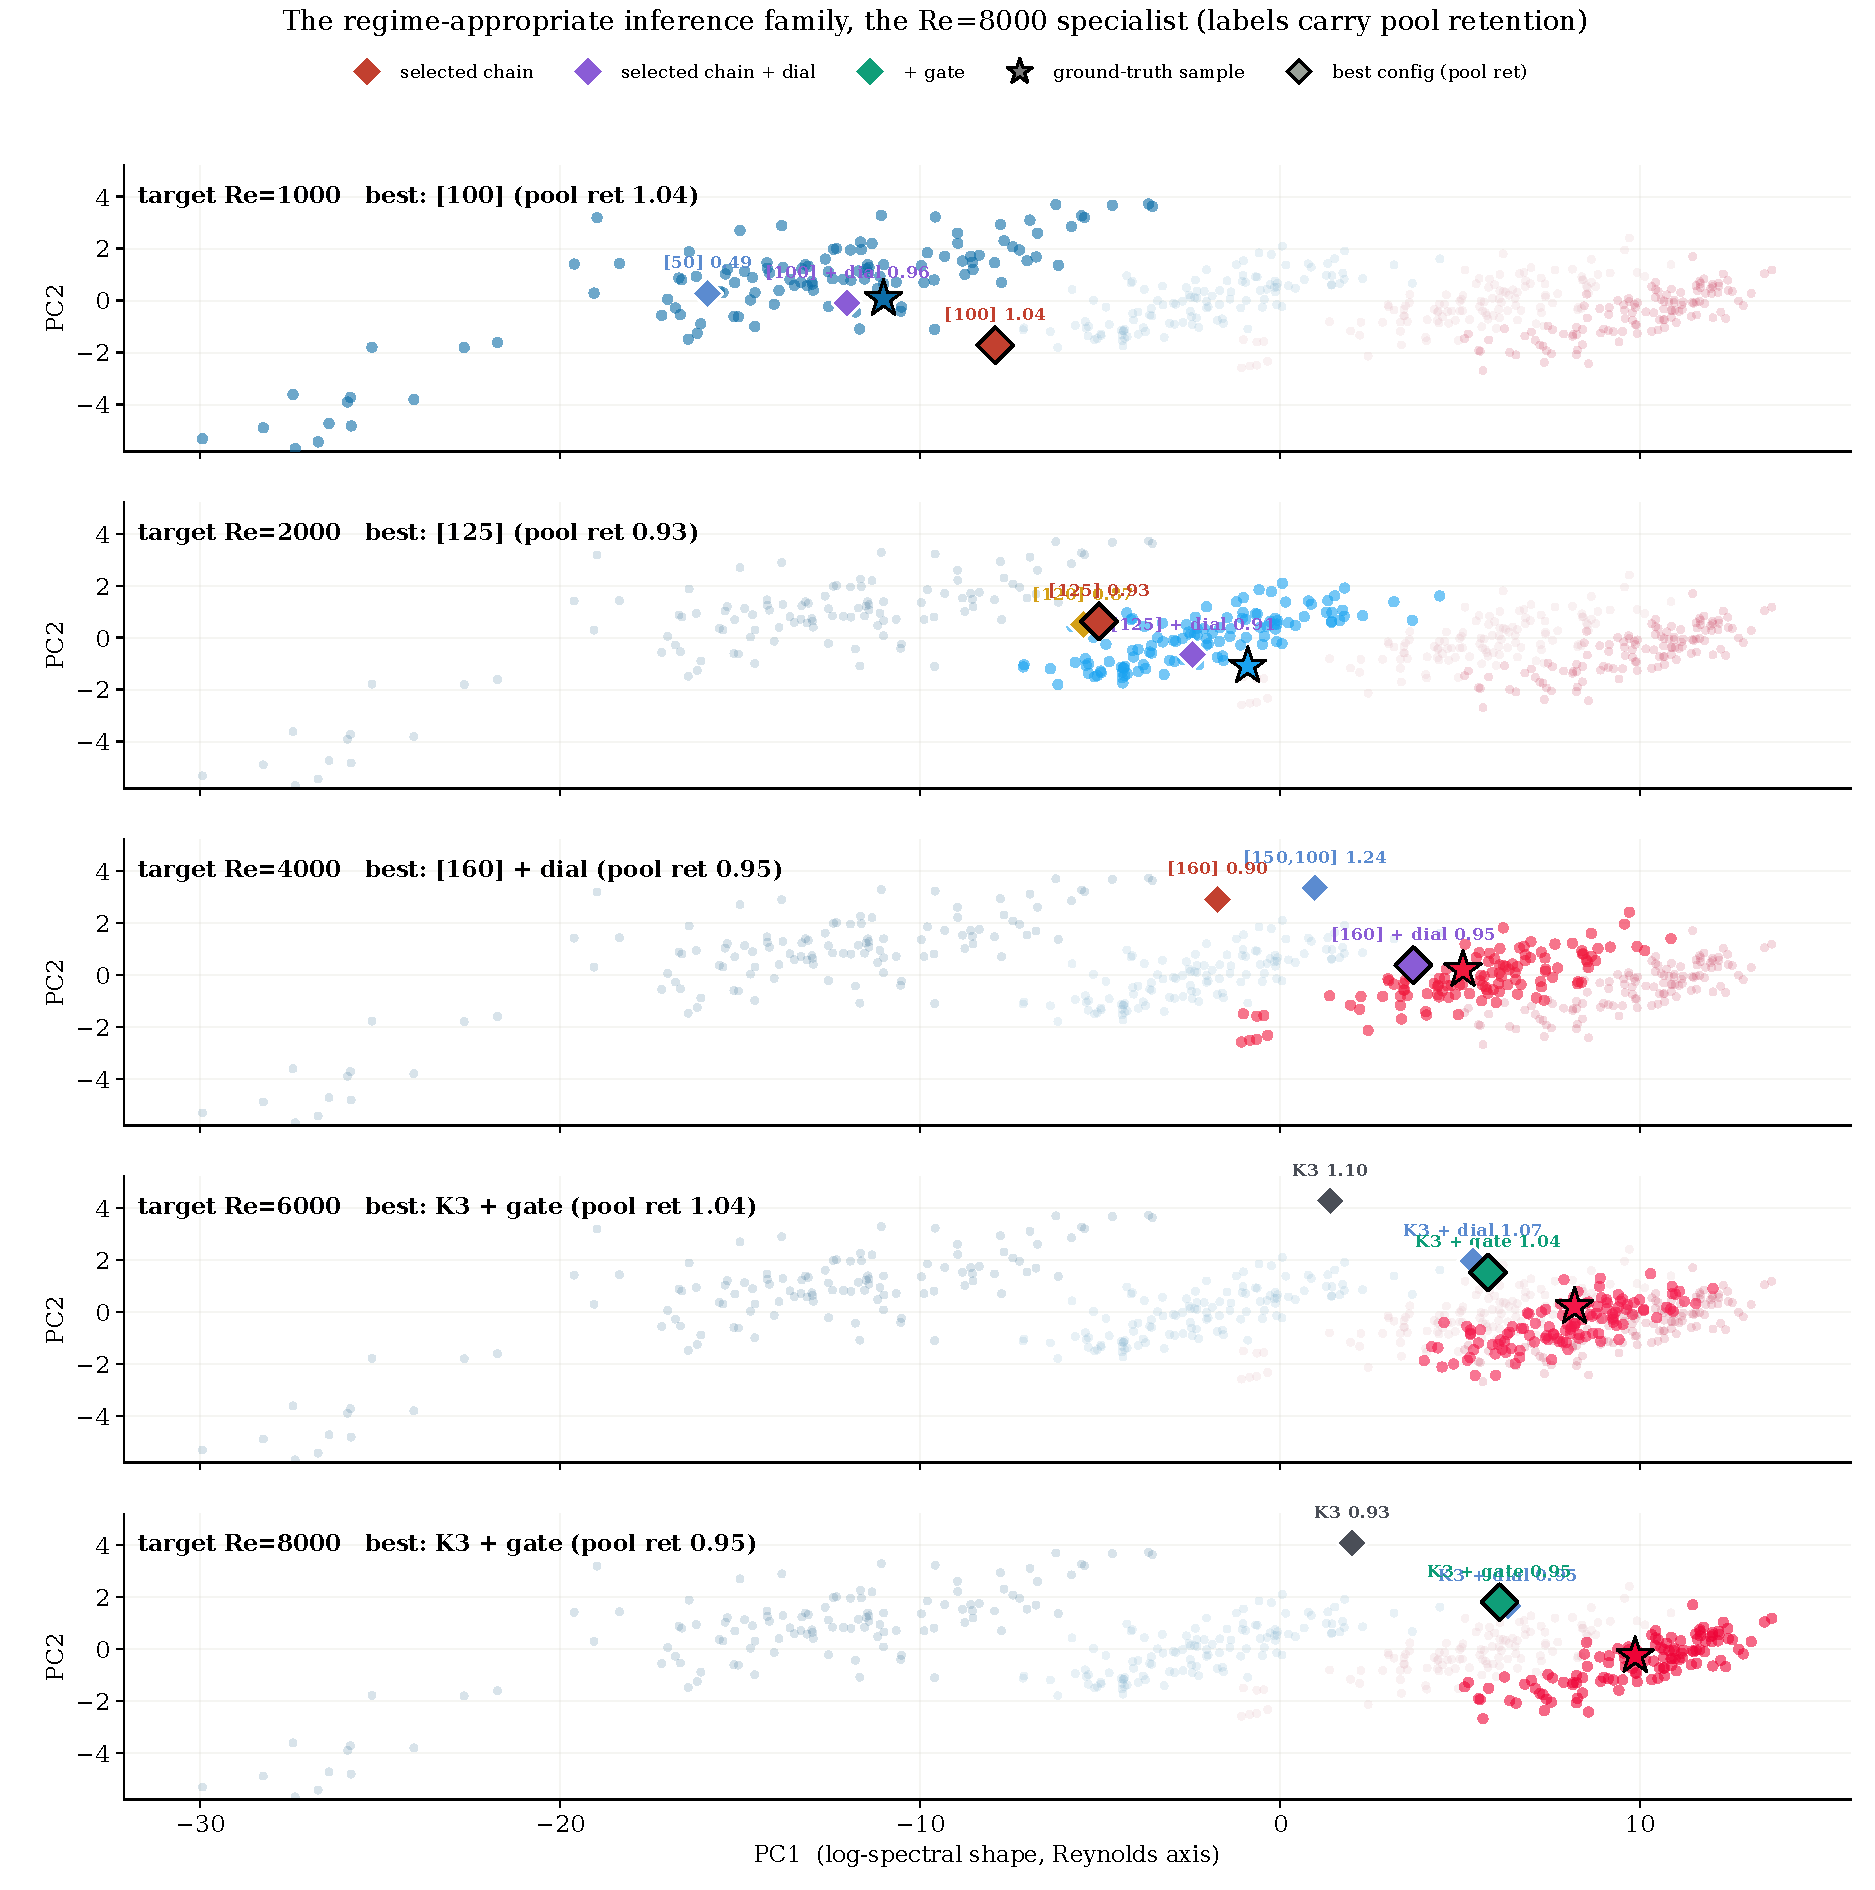
\includegraphics[width=\linewidth]{offmanifold_bestconfig.pdf}
  \caption{The regime appropriate inference family of the $Re=8000$
  specialist at five regimes. Below the home regime the chain family and the
  dialed version of the selected chain, at and above it the full chain with
  the dial and the gate. Labels carry the pool retention and the
  configuration closest to the truth is black edged.}
  \label{fig:bestconfig}
\end{figure}

\begin{figure}[t]
  \centering
  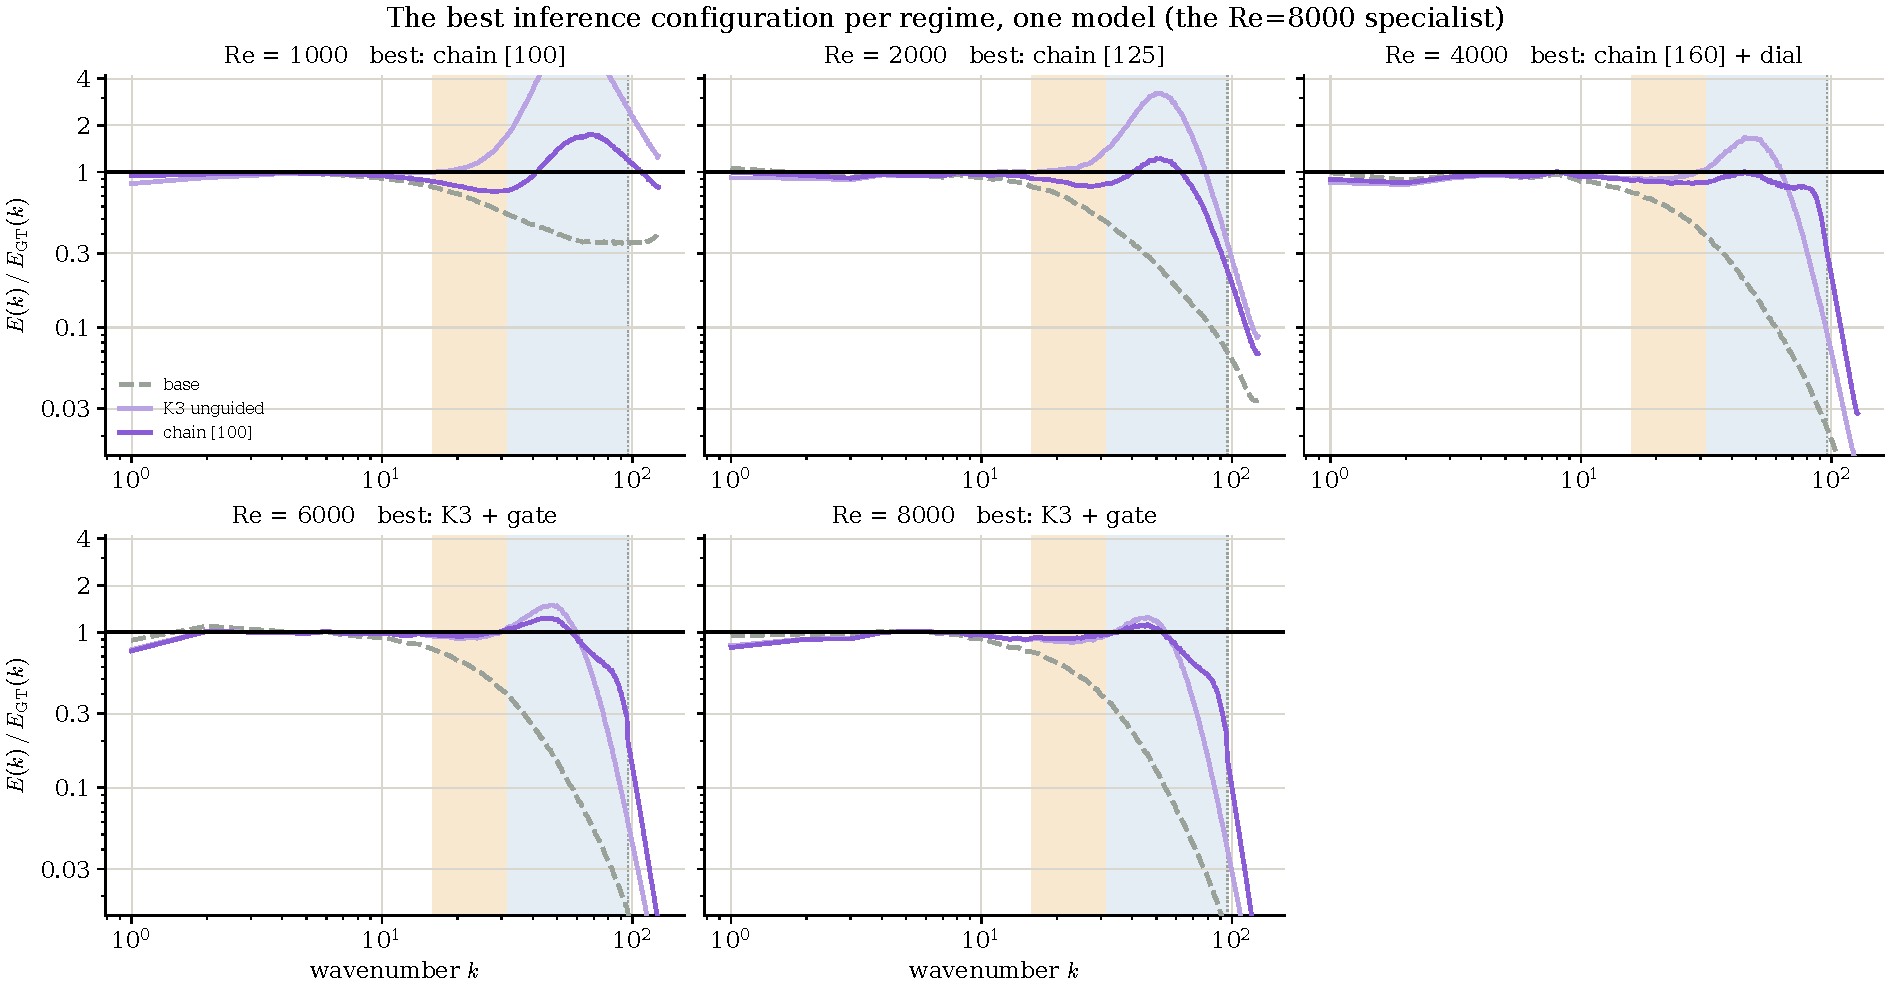
\includegraphics[width=\linewidth]{bestconfig_ratio.pdf}
  \caption{Energy spectrum ratios of the best configuration per regime,
  against the default chain and the base model. Adaptation lands the mid band
  within a small ripple of the truth at every rung, while the highest octave
  collapses in every setting and marks the remaining model ceiling.}
  \label{fig:bestconfig-spectra}
\end{figure}

% ----------------------------------------------------------------------------
\subsection{Toward adaptive guidance, the gate and the gated fine tune}
\label{sec:transfer-gate}

The preceding parts held the guidance fixed and adapted the schedule. The
natural next step is to make the guidance itself adaptive, and this part
presents that step as work in development rather than as a settled method.

The per band gate steers each sample toward its own predicted energy level and
shuts off band by band as the target is reached. With the gate, every model in
the study lands at and above its own training regime, and the gated $Re=8000$
specialist covers the entire upper half of the ladder with retentions between
$0.95$ and $1.04$, which no fixed configuration in this thesis achieves
(Figure~\ref{fig:xfer-gate}). The gate is also the only mechanism in the study
whose correction is decided per sample and per band at inference time, which
is what the attractor result of Section~\ref{sec:transfer-failure} suggests a
complete solution requires.

On the manifold the gate moves the reconstruction cloud in the required
direction. At $Re=8000$ the unguided cloud of the home specialist sits four
units above the arc of physical spectra, an off manifold shape no real regime
has, and nine units short of the true cloud along the Reynolds axis. The gate
returns the cloud to within two units of the arc and roughly halves the
remaining distance to the truth (Figure~\ref{fig:recon-clouds}). The overlap
of the gated cloud with the $Re=4000$ truth in the projection is a
coincidence of the embedding rather than spectral agreement, since the gated
spectra match the $Re=8000$ truth through the mid band and fall below every
regime in the highest octave.

The gate has two demonstrated limits. It cannot create energy a model does
not generate, so gated retention still decays above each model's home, from
$1.04$ at one rung above to $0.74$ when the $Re=1000$ model is pushed to
$Re=8000$. And it cannot fully suppress the overdose far below a model's
home, where the $Re=8000$ specialist still retains $1.38$ at $Re=1000$
against the shortened chain's $1.04$. The gate is therefore a complement to
the chain rather than a replacement for it, strongest exactly where the chain
has nothing further to offer.

Moving the adaptive correction into the weights is the subject of the gated
dose fine tune, in which the gated guidance signal is fed back into training
so that the dose control the gate applies at inference becomes part of the
model itself. Its first results are promising but were obtained on a non
canonical data split, and the rerun on the canonical sequences is left as the
immediate forward direction of this work.

\begin{figure}[t]
  \centering
  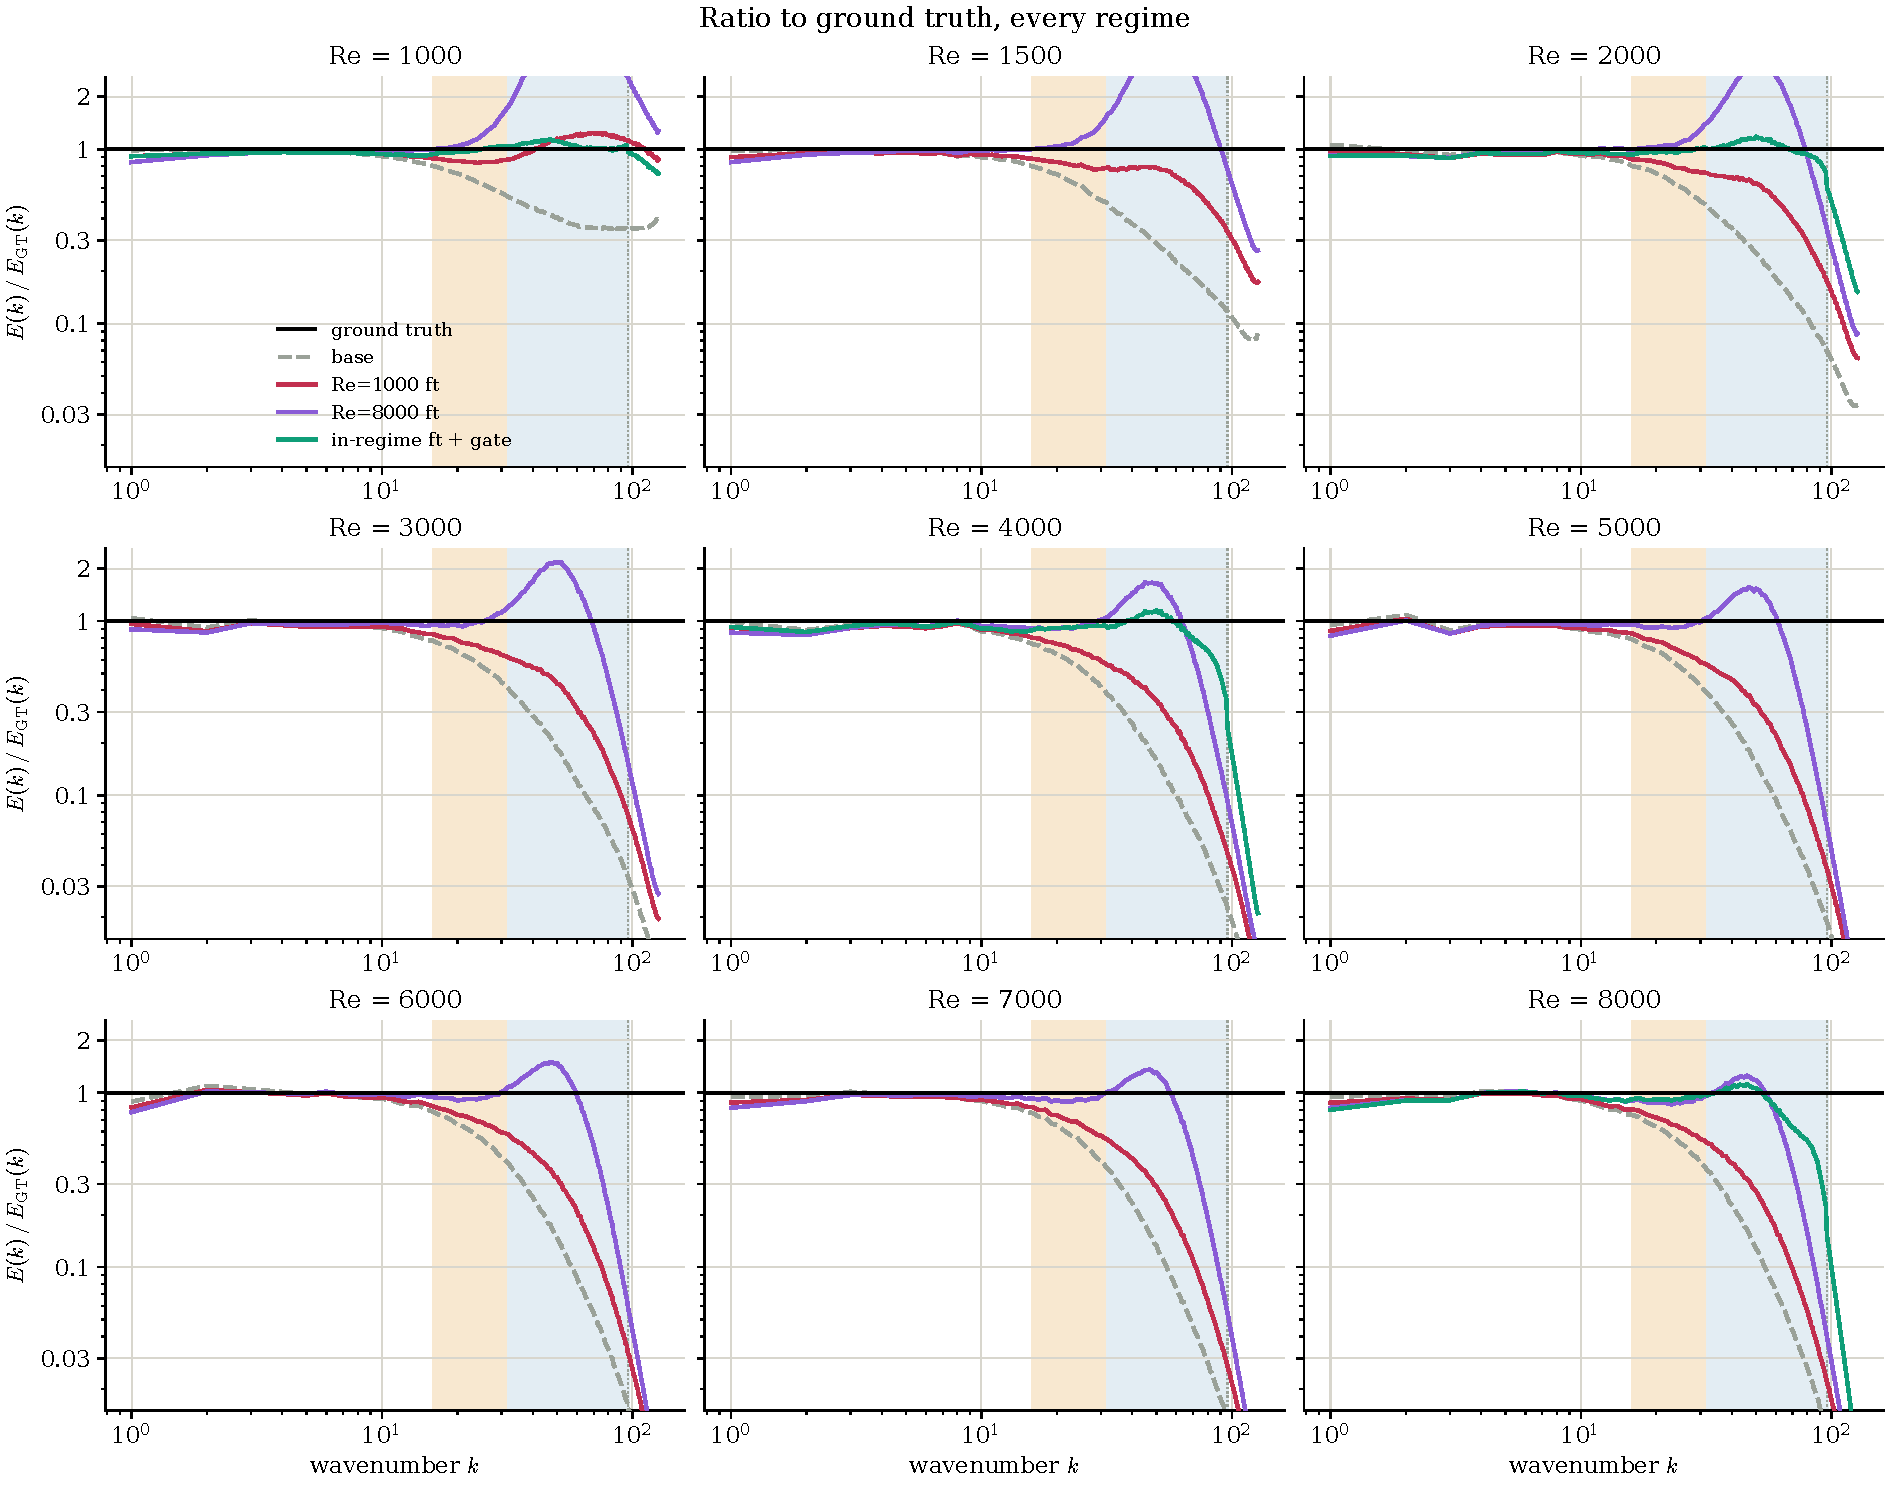
\includegraphics[width=\linewidth]{regime_ratio_dial_xfer.pdf}
  \caption{The two extreme specialists carried across every regime against
  the gated in regime model. The $Re=1000$ model departs the truth at ever
  lower wavenumber as the target rises, the $Re=8000$ model carries one fixed
  surplus bump downward, and the gated in regime model holds the truth line
  through the reward band at every home regime.}
  \label{fig:xfer-gate}
\end{figure}

\begin{figure}[t]
  \centering
  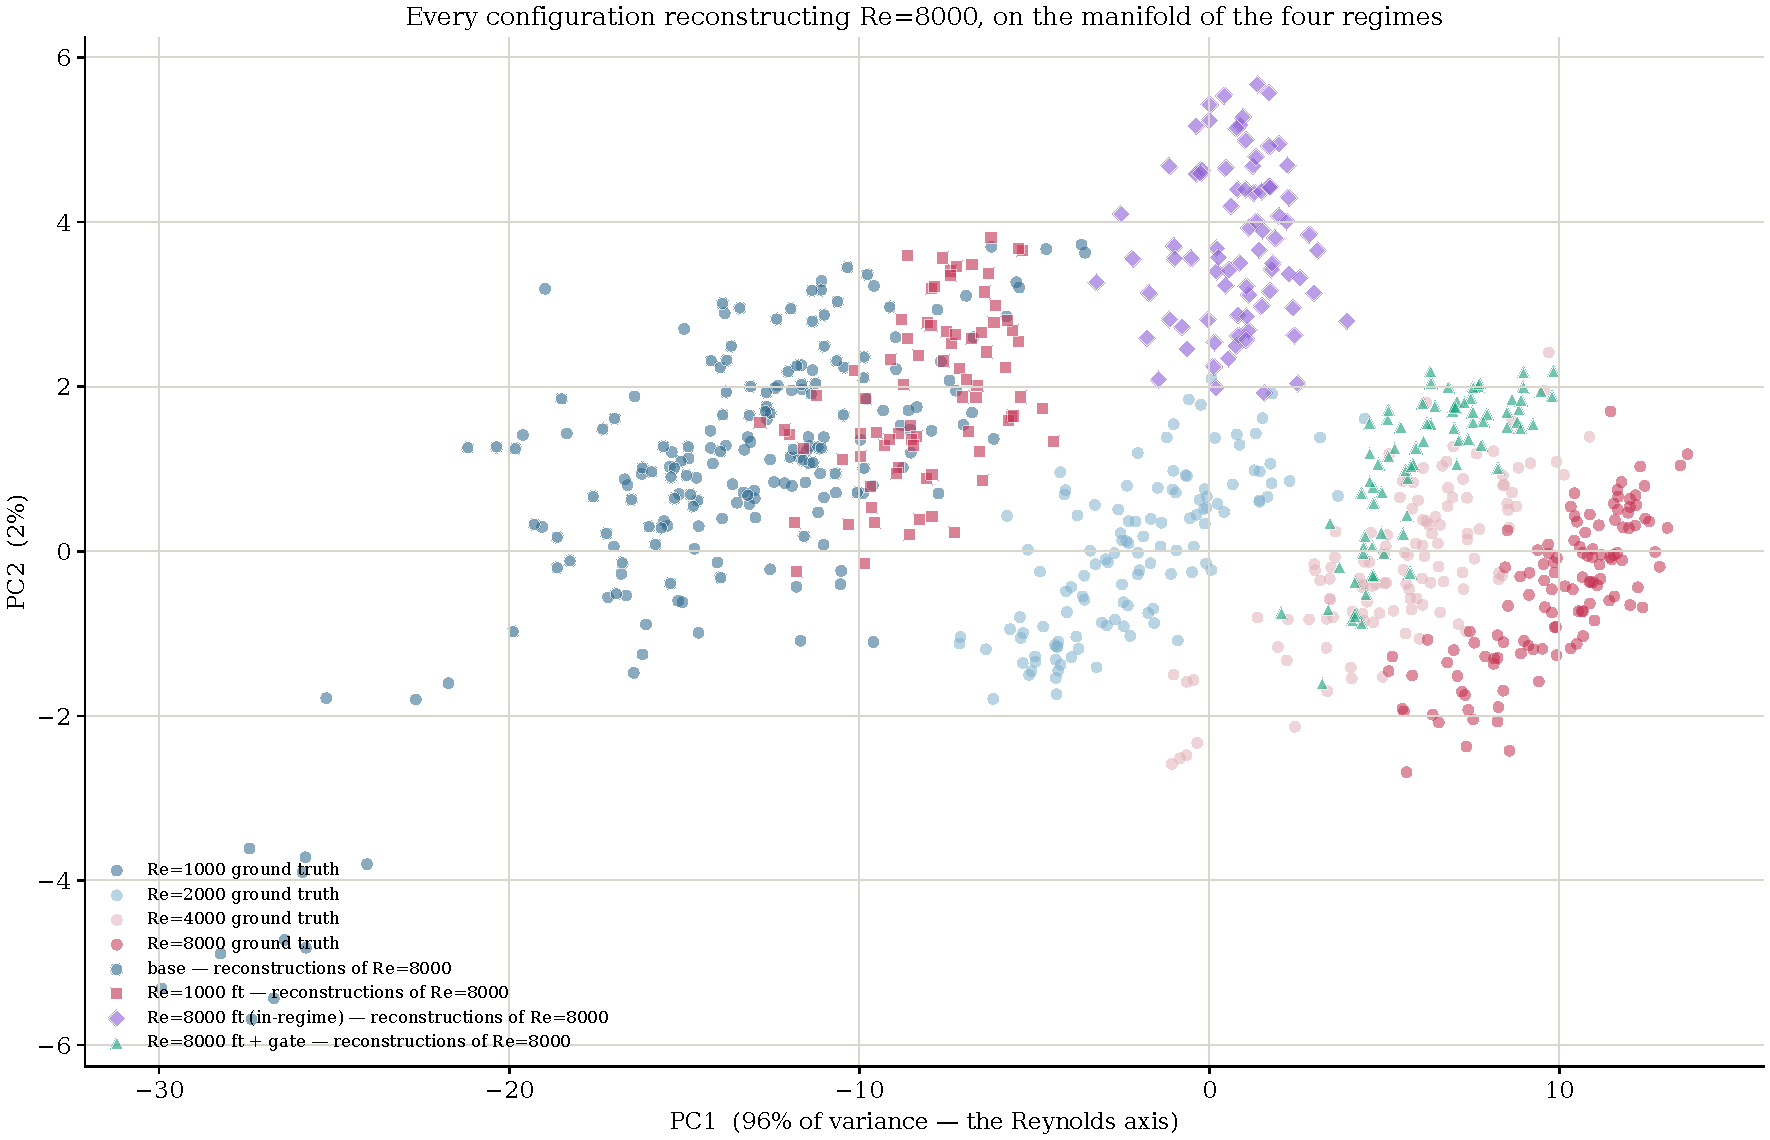
\includegraphics[width=\linewidth]{manifold_recon_clouds.pdf}
  \caption{Every configuration reconstructing $Re=8000$, on the manifold of
  the four regimes. The unguided specialist cloud leaves the arc of physical
  spectra, and the gate returns it toward the arc and roughly halves the
  remaining distance to the true cloud. The residual gap is the missing
  highest octave, and the overlap of the gated cloud with the $Re=4000$
  truth is a projection coincidence rather than spectral agreement.}
  \label{fig:recon-clouds}
\end{figure}

% ============================================================================
% Appendix candidates: offmanifold_passes.pdf, offmanifold_dechain.pdf,
% offmanifold_chainfix.pdf, manifold_chain_clouds.pdf, offmanifold_travel_3d.pdf,
% step_trajectory.pdf, chain_dose.pdf, chain_ladder_spectra.pdf,
% bestconfig_spectra.pdf (absolute), regime_ratio_dial_r4k.pdf,
% regime_ratio_dial_r8k.pdf, regime_pertriplet_gate.pdf, transfer_grid.pdf,
% sample_row_re4000.pdf, offmanifold_topview.pdf (or single panel beside the
% energy trace in the main text).
% ============================================================================
